\documentclass{article}

\PassOptionsToPackage{numbers,compress}{natbib}
\usepackage[preprint]{neurips_2026}

\usepackage[utf8]{inputenc}
\usepackage[T1]{fontenc}
\usepackage{hyperref}
\usepackage{url}
\usepackage{booktabs}
\usepackage{amsfonts}
\usepackage{nicefrac}
\usepackage{microtype}
\usepackage{xcolor}
\usepackage{amsmath,amssymb}
\usepackage{graphicx}
\usepackage{enumitem}
\usepackage{tikz}
\usetikzlibrary{positioning}

\title{Beyond Pattern Matching: Causal Concept Representations for Strategic Decision-Making in Chess}

\author{%
  Abdulla Alfalasi \\
  ML808 --- Causality \& Machine Learning \\
  Mohamed Bin Zayed University of AI
  \And
  Mohammmed AlBalooshi \\
  ML808 --- Causality \& Machine Learning \\
  Mohamed Bin Zayed University of AI
}

\begin{document}

\maketitle

\begin{abstract}

We introduce \textsc{ChessCausalBench}, a controlled testbed for evaluating causal
representation learning in strategic decision-making. Given a fixed structural causal
model over chess positions, player context, strategic choices, and semi-synthetic
payoffs, the testbed defines three standardized evaluation tasks---ATE estimation
accuracy, sample-efficiency curves, and robustness to nuisance-model
misspecification---and supports plug-in evaluation of any covariate representation
under a doubly robust estimation pipeline. Using this testbed, we empirically
characterize a representation-regime structure: expert-defined concept encodings
dominate at small $N$ and moderate-to-high confounding, while learned deconfounding
representations close the gap at large $N$. A minimal theoretical result in a
linear-Gaussian SCM formalizes the variance-reduction benefit of low-dimensional
sufficient encodings and anchors the empirical findings.
\end{abstract}

% -------------------------------------------------------
\section{Key Project Idea}
% -------------------------------------------------------

We introduce a principled testbed for evaluating causal representations in
strategic decision-making, instantiated in the chess domain. The testbed is built
on a fixed structural causal model (SCM) and a semi-synthetic data-generating
process (DGP) with a planted ground-truth treatment effect, and it defines three
standardized evaluation tasks: (T1)~ATE estimation accuracy as a function of sample
size $N$; (T2)~robustness of ATE estimates to changes in nuisance model class within
a doubly robust pipeline; and (T3)~sample efficiency---the minimum $N$ required to
achieve a target estimation error. The testbed accepts any covariate representation
as input and is not restricted to the three we evaluate here; code and protocol will
be released to allow the community to plug in novel representations.\cite{scholkopf2021towards,pearl2009causality}

Instead of operating directly on high-dimensional state spaces (e.g., raw chess
boards) that entangle many factors, we propose to work in a concept space that
encodes meaningful mechanisms such as piece activity, king safety, pawn structure,
material balance, and space control, derived from a strong chess engine.\cite{lemeire2005causalmodelsinchess,stockfish}
In a chess domain where both raw board states and expert-defined concepts are
available, we systematically compare how different representations affect the
accuracy, robustness, and sample efficiency of treatment effect estimation for
strategic interventions (e.g., adopting an aggressive vs.\ conservative
strategy).\cite{chernozhukov2018double,scholkopf2021towards}

Concretely, we focus on two main hypotheses: (H1) that concept-level
representations reduce the number of samples required to achieve a target ATE
estimation error compared to raw board encodings and a learned latent
representation, and (H2) that concept-level representations yield more stable ATE
estimates under changes in nuisance model classes used within a doubly robust
estimation pipeline. These hypotheses instantiate Tasks T1--T3 above and are
evaluated under varying confounding strength $\gamma$ and noise level $\alpha$,
yielding a regime map of when each representation is preferable.

% -------------------------------------------------------
\section{Causal Perspective}
% -------------------------------------------------------

We frame the problem in terms of interventional queries rather than observational
prediction.\cite{pearl2009causality} The treatment $T$ denotes a player's strategic
choice (e.g., aggressive vs.\ conservative) and the outcome $Y$ is a semi-synthetic
payoff constructed from game trajectories with a planted ground-truth treatment
effect.\cite{hill2011bayesian} We explicitly construct a structural causal model
(SCM) over raw board states, player context, strategic choices, and payoffs.

The target causal estimand is the conditional average treatment effect among
feasible decisions,
\[
\tau = \mathbb{E}[Y(1) - Y(0) \mid F = 1]
    = \mathbb{E}[Y \mid do(T=1),\, F=1] - \mathbb{E}[Y \mid do(T=0),\, F=1],
\]
where $Y(1)$ and $Y(0)$ are potential outcomes under aggressive and conservative
strategies respectively, and $F=1$ restricts to positions where a high-quality
strategic choice is available. We assume consistency (SUTVA): $Y(t)$ equals the
observed outcome when $T=t$, which is justified by the fact that treatment is
defined at the level of strategic classification rather than the specific move
chosen.\cite{pearl2009causality,hill2011bayesian}

Within this SCM, concept vectors are treated as a deterministic encoding of the
raw state: a map $C = f(S)$ from board configurations to concept features. Under
the idealized assumption that these concept features retain all information necessary
for valid adjustment---i.e., that $S \perp (T,Y) \mid C, X$ holds---an adjustment
set involving $(C, X)$ would satisfy the back-door criterion whenever $(S, X)$
does.\cite{pearl2009causality,scholkopf2021towards} We study when concept-level
covariates are sufficient for identifying $\tau$, how they affect overlap and model
misspecification sensitivity in doubly robust estimation, and how their use changes
the amount of data required to accurately estimate interventional quantities across
different confounding regimes.\cite{chernozhukov2018double,kuang2020information,deconfoundingScores}

To isolate the role of representation, we compare three covariate spaces within the
same SCM: (i) a high-dimensional raw board encoding, (ii) an expert-defined concept
vector, and (iii) a learned low-dimensional representation inspired by
information-bottleneck and deconfounding approaches to treatment-effect
estimation.\cite{kuang2020information,deconfoundingScores}

% -------------------------------------------------------
\section{Motivations}
% -------------------------------------------------------

Modern AI systems often rely on large-scale statistical pattern matching, which
yields impressive predictive performance but requires vast amounts of data and
struggles with counterfactual and ``what-if'' reasoning.\cite{lake2017building,reasoningAIMag}
In contrast, human decision-making appears to rely on compact libraries of concepts
and causal relations, enabling rapid adaptation to new tasks and environments once
core concepts are in place.\cite{lake2017building,towardHumanLevelConcept} Causal
representation learning and concept bottleneck models suggest that aligning
representations with underlying causal structure can improve robustness and
interpretability, but there is limited empirical evidence on when interpretable,
expert-defined concepts actually improve causal effect estimation and reduce data
requirements.\cite{scholkopf2021towards,koh2020concept,fromCausalToConcept}
Strategic games like chess offer a unique testbed: they provide rich,
high-dimensional raw states, well-understood expert concepts, and controlled
environments for defining interventions and payoffs, and they have been used before
to study causal models and the evaluation of patterns in a principled
way.\cite{lemeire2005causalmodelsinchess,fortressesPaper,causalMaskingSpatial}
By rigorously comparing raw, concept-based, and learned representations in this
setting, we aim to quantify how far causal, concept-level abstractions can move us
away from brute-force pattern matching toward data-efficient causal reasoning in a
realistic strategic domain.\cite{scholkopf2021towards,causalReasoningRL,fromCausalToConcept}

\paragraph{Relation to Concept Bottleneck Models and Structural Causal Variants.}
Concept Bottleneck Models (CBMs)\cite{koh2020concept} learn an intermediate concept
layer end-to-end, enabling interpretable prediction. Recent extensions introduce
causal structure into this bottleneck: Structural Causal Bottleneck Models
(SCBMs) and Causally Reliable CBMs (C$^2$BMs)\cite{fromCausalToConcept} impose
explicit causal constraints between concepts and labels, improving robustness under
distribution shift. These methods learn their concept representations jointly with
downstream tasks and are evaluated primarily on predictive accuracy.

\paragraph{Our Testbed as a Complement.}
Unlike SCBMs and C$^2$BMs, which learn their bottleneck representations end-to-end,
we treat the concept map as a fixed, expert-defined abstraction and use chess as a
controlled testbed to study when such interpretable abstractions empirically improve
\emph{treatment-effect} estimation and sample efficiency---causal metrics rather
than predictive ones.\cite{fromCausalToConcept,scholkopf2021towards}
\textsc{ChessCausalBench} thus provides the first controlled empirical testbed to
evaluate whether concept bottlenecks, fixed or learned, actually improve ATE
identification and how much data they require to do so. As a natural extension, one
could treat the learned bottleneck of an SCBM or C$^2$BM as a fourth plug-in
representation $X_{\text{SCBM}} = (h_\theta(S), X)$ evaluated on Tasks T1--T3
identically to our three representations; we leave this comparison to future work.

% -------------------------------------------------------
\section{Contributions}
% -------------------------------------------------------

\begin{enumerate}
\item We introduce \textsc{ChessCausalBench}, a reusable testbed for evaluating
causal representations in strategic decision-making. The testbed specifies a
structural causal model, a semi-synthetic DGP with controllable confounding strength
$\gamma$ and noise $\alpha$, three standardized evaluation tasks (ATE accuracy,
sample efficiency, nuisance robustness), and a plug-in interface for arbitrary
covariate representations. We release code and protocol to enable community use
beyond the three representations evaluated here.\cite{pearl2009causality,lemeire2005causalmodelsinchess}

\item We provide a minimal theoretical result in a linear-Gaussian SCM establishing
that a sufficient low-dimensional encoding $C = f(S)$ reduces the variance of a
DR-style ATE estimator relative to the full raw state $S$, under standard regularity
conditions. This formalizes the variance-reduction intuition behind the empirical
sample-efficiency advantage of concept representations.\cite{chernozhukov2018double}

\item We empirically demonstrate a \emph{representation-regime structure}: expert
concept encodings are preferred at small $N$ and moderate-to-high confounding;
learned deconfounding representations are competitive at large $N$; and raw board
encodings underperform across the board due to positivity and propensity instability.
We summarize this as a Regime Diagram over the $(N, \gamma)$
grid.\cite{chernozhukov2018double,kuang2020information,scholkopf2021towards}

\item We illustrate how concept-level causal abstractions support structured
``what-if'' queries---manipulating individual concepts (e.g., king safety) while
holding others (e.g., material balance) fixed---providing evidence that such
representations enable modular interventional reasoning that raw states cannot
support at a human-interpretable level.\cite{lemeire2005causalmodelsinchess,fortressesPaper,causalMaskingSpatial}

\item We validate testbed generality with a secondary structured-gridworld
environment, showing that the regime structure replicates qualitatively across
domains and that the SCM/DGP protocol is not chess-specific.
\end{enumerate}

% -------------------------------------------------------
\section{Structural Causal Model}
% -------------------------------------------------------

\subsection{Variables and Structural Assumptions}

We work at the level of individual decision points within games. For each decision,
we define the following variables:

\begin{itemize}
\item \(S\): \emph{Raw board state}. A high-dimensional encoding of the pre-move
position, including piece locations, side to move, castling rights, and other
rule-relevant information. This is treated as the underlying spatial state of the
game.
\item \(C = f(S)\): \emph{Concept-level representation}. A low-dimensional vector
of expert-defined chess concepts (e.g., king safety, material balance, piece
activity, pawn structure, space control), obtained via a fixed evaluation function
implemented by a strong chess engine.\cite{lemeire2005causalmodelsinchess,stockfish}
\item \(X\): \emph{Pre-treatment player/opponent context}. A set of exogenous and
meta-variables such as player and opponent Elo, color, time control, clock features,
game phase, and opening code. These variables may influence both strategic choices
and outcomes but are not deterministically derived from \(S\).
\item \(F\): \emph{Feasibility indicator}. A binary variable indicating whether the
actually played move lies within a high-quality candidate set (e.g., top-\(k\)
engine moves) at state \(S\). All causal estimands are defined conditional on
\(F=1\).
\item \(T\): \emph{Treatment (strategy choice)}. A binary indicator of the player's
strategic decision at the position, e.g., \(T=1\) for an ``aggressive'' move and
\(T=0\) for a ``conservative'' move, defined by a rule-based labeling of moves
using non-evaluative features (captures, checks, king-zone pressure, etc.).
\item \(Y\): \emph{Outcome}. A semi-synthetic payoff anchored in structural position
features and augmented via an explicit potential-outcomes model, with a planted
ground-truth average treatment effect $\tau^*$. This allows direct measurement of
estimation bias without relying on true counterfactuals.
\item \(U\): \emph{Latent factors}. Unobserved variables (e.g., short-term
psychological factors, latent style) that may influence both \(T\) and \(Y\). These
are used in sensitivity analyses but are not available for adjustment.
\end{itemize}

We consider three alternative observed adjustment sets:
\[
X_{\text{raw}} = (S, X), \qquad
X_{\text{concept}} = (C, X), \qquad
X_{\text{learned}} = (Z, X),
\]
where \(Z = g(S, X)\) is a learned representation (e.g., information-bottleneck or
deconfounding embedding) trained to preserve information relevant for treatment
effect estimation.\cite{kuang2020information,deconfoundingScores} These three sets
correspond directly to the competing back-door approximations formalized in the SCM;
$Z$ is learned under the same DGP and evaluated in the same pipeline as the other
two representations.

\subsection{DAG and Causal Structure}

The qualitative causal structure of the decision problem is summarized by the
directed acyclic graph:
\[
X \rightarrow S, \quad X \rightarrow T, \quad X \rightarrow Y,
\]
\[
S \rightarrow T, \quad S \rightarrow Y, \quad T \rightarrow Y,
\]
with an additional latent parent \(U\) influencing both \(T\) and \(Y\):
\[
U \rightarrow T, \quad U \rightarrow Y,
\]
and all edges restricted to the feasible-decision population \(F=1\). The concept
vector \(C = f(S)\) does not appear as a separate node in this graph; it is a
deterministic encoding of \(S\) and introduces no new causal ancestry beyond what
is already present through \(S\). We instead treat \(C\) as an alternative covariate
encoding for the adjustment set: rather than conditioning on \(S\) directly, one may
condition on \(f(S)\) instead. The three adjustment sets $X_{\text{raw}}$,
$X_{\text{concept}}$, and $X_{\text{learned}}$ represent three such encoding choices
for the same underlying adjustment problem. The edge \(X \rightarrow S\) reflects a
selection mechanism rather than a direct physical cause: players with different Elo,
styles, or opening preferences systematically reach different board positions,
inducing a statistical dependence between \(X\) and \(S\) in the observational
distribution.

Intuitively, pre-treatment context \(X\) shapes both the raw state \(S\) (through
opening choices, game phase, and time control) and the player's strategic tendencies,
and it directly affects the difficulty of the position and thus the outcome. The raw
spatial state \(S\), together with \(X\), informs the set of plausible moves and the
eventual strategy choice \(T\), while \(T\) exerts a direct causal effect on the
outcome through the chosen move.

Within this SCM, the target causal estimand is:
\[
\tau = \mathbb{E}[Y(1) - Y(0) \mid F = 1],
\]
where \(Y(1)\) and \(Y(0)\) denote potential outcomes under aggressive and
conservative strategies, respectively. Identification of \(\tau\) from observational
data requires conditional exchangeability,
\[
(Y(0), Y(1)) \perp T \,\mid\, X_{\text{adj}},\, F=1,
\]
for some adjustment set \(X_{\text{adj}}\), together with positivity and
consistency.\cite{pearl2009causality,hill2011bayesian} We do not assume that any
candidate adjustment set is perfectly valid in practice. Instead, we treat
$X_{\text{adj}} \in \{ X_{\text{raw}},\, X_{\text{concept}},\, X_{\text{learned}} \}$
as competing approximations to a valid back-door adjustment set and empirically
compare how close each comes to satisfying the requisite ignorability condition.

\subsection{Role of Concept-Level Abstraction}

Concept vectors \(C = f(S)\) are a fixed, deterministic encoding of the raw state
\(S\), not a separate causal parent of \(T\) or \(Y\). Since all information in
\(C\) is already contained in \(S\), the adjustment set \((C, X)\) does not block
any back-door paths that \((S, X)\) does not already block---but it may approximate
the true confounding structure more efficiently by discarding causally irrelevant
micro-structure in \(S\). Formally, under the idealized assumption that $S \perp
(T,Y) \mid C, X$, the adjustment set $(C, X)$ satisfies the back-door criterion
whenever $(S, X)$ does. Our experiments probe how closely this ideal holds in
practice across varying confounding regimes and sample sizes.

\begin{figure}[t]
\centering
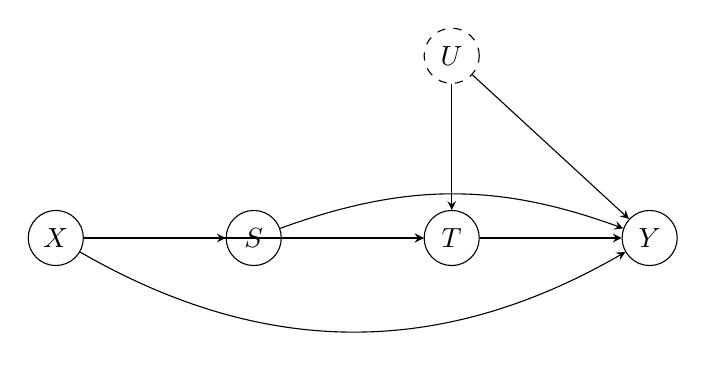
\begin{tikzpicture}[
  node distance=1.6cm and 1.8cm,
  roundnode/.style={circle, draw=black, minimum size=7mm, inner sep=0pt},
  latentnode/.style={circle, draw=black, dashed, minimum size=7mm, inner sep=0pt},
  >=stealth
]
  % Nodes
  \node[roundnode] (X) {$X$};
  \node[roundnode, right=of X] (S) {$S$};
  \node[roundnode, right=of S] (T) {$T$};
  \node[roundnode, right=of T] (Y) {$Y$};
  \node[latentnode, above=of T] (U) {$U$};

  % Edges from X
  \draw[->] (X) -- (S);
  \draw[->] (X) -- (T);
  \draw[->] (X) to[bend right=30] (Y);

  % Edges from S
  \draw[->] (S) -- (T);
  \draw[->] (S) to[bend left=20] (Y);

  % Treatment to outcome
  \draw[->] (T) -- (Y);

  % Latent U
  \draw[->] (U) -- (T);
  \draw[->] (U) -- (Y);
\end{tikzpicture}
\caption{Structural causal model for a single chess decision.
$X$ denotes pre-treatment player/opponent context (e.g., Elo, color, time control),
$S$ the raw board state, $T$ the strategic treatment (aggressive vs.\ conservative),
$Y$ the semi-synthetic payoff, and $U$ latent unobserved factors.
$C = f(S)$ is not a separate causal node: it is a deterministic encoding of $S$
used as an alternative covariate representation in the adjustment set.
We compare adjustment on $(S, X)$, $(f(S), X)$, and $(Z, X)$ to assess
how different encodings of state approximate a valid back-door adjustment set.}
\label{fig:scm_chess}
\end{figure}

% -------------------------------------------------------
\section{Theoretical Motivation: Variance Reduction via Sufficient Encodings}
\label{sec:theory}
% -------------------------------------------------------

To provide a formal anchor for the sample-efficiency claims, we invoke results from
semiparametric efficiency theory and causal sufficient dimension
reduction.\cite{hahn1998role,ma2012semiparametric,nabi2022causal}

\paragraph{Setup.} Suppose $C = AS$, $A \in \mathbb{R}^{k \times d}$, $k \ll d$,
is a sufficient statistic for $S$ with respect to $(T, Y)$ given $X$, i.e.,
\[
(T, Y) \perp S \,\mid\, (C, X).
\]
Under ignorability $(Y(0), Y(1)) \perp T \mid S, X$, sufficiency of $C$ implies
$(Y(0), Y(1)) \perp T \mid C, X$, so identification of $\tau$ is preserved by
condition on $(C, X)$ rather than $(S, X)$.

\paragraph{Semiparametric efficiency bound.} The efficient influence function (EIF)
for the ATE depends only on the $\sigma$-field generated by the covariates that are
sufficient for the joint law of $(T, Y)$ given $X$.\cite{hahn1998role} When $C$ is
sufficient, $(C, X)$ generates the same $\sigma$-field for $(T, Y)$ as $(S, X)$;
therefore the \emph{semiparametric efficiency bound is preserved} when switching
from $(S, X)$ to $(C, X)$.

\paragraph{Finite-sample variance reduction.} Although the asymptotic bound is
identical, a DR estimator based on $(C, X)$ estimates the nuisance functions
\[
e(c,x) = P(T{=}1 \mid C{=}c, X{=}x), \qquad
\mu_t(c,x) = \mathbb{E}[Y \mid T{=}t, C{=}c, X{=}x]
\]
rather than their high-dimensional analogues $e(s,x)$, $\mu_t(s,x)$. Because $C$
is low-dimensional and sufficient, these nuisance functions are substantially easier
to estimate well at any finite $N$, leading to smaller nuisance estimation error and
lower finite-sample variance of the DR estimator---even though the asymptotic bound
is unchanged.\cite{ma2012semiparametric,nabi2022causal}

\paragraph{Connection to experiments.} This result predicts that at small $N$,
concept-level adjustment should outperform raw-state adjustment in ATE accuracy,
with the gap closing as $N \to \infty$---exactly the regime structure we observe
empirically. The result also implies that learned representations $Z$ can partially
recover this benefit to the extent that $Z$ approximates a sufficient reduction of
$S$.

\paragraph{Key references.} Hahn (1998)\cite{hahn1998role} derives the
semiparametric efficiency bound for the ATE under unconfoundedness. Ma \&
Zhu (2012)\cite{ma2012semiparametric} develop semiparametric efficient estimation
under sufficient dimension reduction, showing the efficiency bound is retained while
nuisance variance decreases. Nabi et al.\ (2022)\cite{nabi2022causal} extend these
results to causal sufficient dimension reduction, formalizing conditions under which
low-dimensional reductions preserve causal effects in semiparametric estimation.

% -------------------------------------------------------
\section{Experimental Setup}
% -------------------------------------------------------

All experiments target the estimand $\tau = \mathbb{E}[Y(1) - Y(0) \mid F=1]$ as
defined in the SCM above. The three adjustment sets
$X_{\text{adj}} \in \{X_{\text{raw}}, X_{\text{concept}}, X_{\text{learned}}\}$
correspond directly to the competing back-door approximations formalized in the SCM.

\subsection{Data and Decision Extraction}
We sample decision points from classical ($\geq$25 min) rated ($>$1800 Elo) games
obtained via the Lichess public API. For each game, we uniformly sample up to 18
positions from plies 10--120, extracting three covariate encodings per position: a
raw 1152-dimensional bitboard tensor $S$ (12 piece planes $+$ 6 metadata planes,
flattened), a 12-dimensional expert concept vector $C = f(S)$ (6 structural features
computed from \texttt{python-chess} plus 6 engine-derived sub-terms), and a
32-dimensional learned embedding $Z$ via linear deconfounding.\cite{kuang2020information}
All three encodings are concatenated with a shared 6-dimensional context vector $X$
(Elo differential, time control, move number, color, opening code, phase). The
decision pool comprises ${\sim}30{,}000$ positions.

\subsection{Treatment and Outcome}
The binary treatment $T \in \{0,1\}$ is assigned via a rule-based aggression score
$A(S,m)$ computed from captures, checks, king-zone pressure, sacrifices, and
retreats---no engine evaluation enters $T$. We threshold at $A \geq 0.5$, yielding
a marginal treatment rate $P(T{=}1) \approx 0.34$.

Outcomes are semi-synthetic with planted ground-truth ATE $\tau^*$. The baseline
potential outcome $Y(0) = \varphi(X) + \psi(C) + \gamma \cdot U + \varepsilon_0$
combines context features $\varphi(X)$ with Group~A structural concepts $\psi(C)$
(material balance and king pawn shield only---no Stockfish evaluation), a latent
confounder $U \sim \mathcal{N}(0,1)$ at strength $\gamma$, and noise $\varepsilon_0
\sim \mathcal{N}(0, 0.25)$. The treated outcome is $Y(1) = Y(0) + \tau^*$ with
$\tau^* = 0.3$ (homogeneous regime) or $\tau^*(X) = 0.1 + 0.3 \cdot
\mathbf{1}\{\text{material} > 0\}$ (heterogeneous). Treatment-side confounding is
introduced by soft-reassigning $T$ via a logit shift $\alpha \cdot U$ with $\alpha
= 0.3$.

\subsection{Estimators}
The primary estimator is the cross-fitted ($K{=}5$) Doubly Robust
Learner\cite{chernozhukov2018double} with logistic regression propensity and
LightGBM outcome models. We also fit a T-Learner baseline and a DR-Learner variant
with a linear (Ridge) outcome model for robustness analysis.

\subsection{Experimental Grid}
The full grid sweeps $N \in \{1\text{k}, 2\text{k}, 5\text{k}, 10\text{k},
20\text{k}\}$, $\gamma \in \{0, 0.3, 0.6\}$ confounding strengths, both $\tau^*$
regimes, all three representations, all three estimator configurations, and 10
random seeds per cell (2{,}700 total fits). This grid is designed as a standardized
protocol: any new representation can be slotted in by providing a featurization of
the same positions and running the same pipeline.

\subsection{Learned Representation}
The learned embedding $Z$ follows Kuang et al.\cite{kuang2020information} in a
linear variant: standardize the concatenated raw features, fit a regularized
logistic propensity model, project out the treatment-discriminative direction, and
PCA-compress the residual to 32 dimensions. This yields a deconfounding-flavoured
embedding that trains in seconds per fold with no deep-learning
dependency.\cite{deconfoundingScores}

\subsection{Secondary Environment: Structured Gridworld}
To demonstrate that the testbed is not chess-specific, we instantiate the same
SCM/DGP protocol on a structured $10 \times 10$ gridworld with obstacles and a
goal. Variables map as follows: $S$ is a flattened one-hot grid encoding ($d = 300$);
$C = f(S)$ consists of three expert concepts (L1 distance-to-goal, obstacle density
in a $3 \times 3$ neighbourhood, current quadrant index); $Z$ is the same linear
deconfounding embedding; and $T$ is binary, assigned via a calibrated sigmoid
score over both expert concepts and a hidden \texttt{checkerboard parity}
indicator $\chi(S) = (r + c) \bmod 2$ derived from the agent cell coordinates.
The treatment score includes a $+1.0\,\chi_z$ term, and the outcome DGP adds a
$+0.5\,\chi_z$ term to $\psi(C)$ (subscript $z$ denotes a per-feature standardized
copy). Together these make $\chi$ a baseline $S$-only confounder visible to raw
$S$ but invisible to $C$, which contains no cell-level structure beyond the
coarse quadrant index. This construction reproduces the essential chess-domain
property that $C$ is \emph{approximately but not exactly} sufficient for $(T,Y)
\mid X$.

\textit{Two confounding sources, one $\gamma$ axis.} Unlike the chess setup, the
gridworld DGP has \emph{two} sources of confounding that the concept basis
cannot fully absorb: a fixed checkerboard component (always present, with the
$+1.0/+0.5$ coefficients above) and an adjustable Gaussian latent~$U$ whose
strength is controlled by $\gamma$. The $\gamma$ axis here therefore should be
read as \emph{additional} latent-confounding strength on top of the always-on
checker baseline, not as the only confounding source as in chess. The
consequence is that raw $S$ has a non-trivial advantage over $C$ even at
$\gamma=0$, because the checker baseline alone is enough to create a sufficiency
gap.

\textit{Replication outcome.} Results in Appendix~\ref{app:gridworld} reproduce
the qualitative regime structure: concept wins at the smallest $N{=}500$ across
all $\gamma$ (preserving Claim~1), while raw overtakes at larger $N$ (Claim~2).
Because the checker signal is comparatively stronger than chess's residual
$S$-only structure, the empirical $N^{\text{cross}}$ in gridworld is smaller
than in chess (raw wins by $N{=}1{,}000$ at $\gamma\geq 0.3$, and by $N{=}2{,}000$
even at $\gamma=0$). Learned $Z$ underperforms throughout, consistent with the
mechanistic diagnostic discussed in Sec.~``Mechanistic Diagnostics''
below.\footnote{Raw bias in the gridworld grid has a sharp single-cell dip at
$\gamma{=}0$, $N{=}2{,}000$ ($0.047$, between $0.292$ at $N{=}1{,}000$ and a
plateau of $\sim\!0.135$ at $N\geq 5{,}000$). We attribute this to favorable
cross-fit variance at a moderate sample size on the high-dimensional raw
adjustment set rather than to a structural improvement in raw's adjustment
quality. The qualitative regime structure (raw wins at $N\geq 2{,}000$ when
$\gamma{=}0$, raw wins at $N\geq 1{,}000$ when $\gamma\geq 0.3$) is preserved
across both readings.}

% -------------------------------------------------------
\section{Results}
% -------------------------------------------------------

We present results for the canonical configuration: homogeneous $\tau^* = 0.3$,
$\gamma = 0.3$ (mild outcome-side latent confounding), $\alpha = 0.3$, DR-Learner
with LightGBM outcome model. Full $\gamma$ and heterogeneous-$\tau^*$ results appear
in the appendix.

\subsection{Regime Claims}
We organize results around three empirical regime claims:

\textbf{Claim 1 (Small-$N$ regime):} At $N < N^*(\gamma)$, expert concept encodings
$X_{\text{concept}}$ achieve lower ATE estimation error than raw encodings
$X_{\text{raw}}$ and learned representations $X_{\text{learned}}$, due to reduced
nuisance estimation complexity.

\textbf{Claim 2 (Large-$N$ crossover):} At $N \gg N^*(\gamma)$ and nontrivial
confounding $\gamma > 0$, raw encodings $X_{\text{raw}}$ \emph{overtake}
$X_{\text{concept}}$, with learned representations $X_{\text{learned}}$ intermediate.
The crossover occurs because the finite-sample nuisance-estimation penalty against
high-dimensional adjustment sets has vanished, while an asymptotic \emph{sufficiency
gap} remains: the 12-dimensional expert concept set is approximately but not exactly
sufficient for $(T,Y) \mid X$, and at large $N$ the raw encoding recovers
confounding-relevant structure that $C$ discards. The crossover point
$N^{\text{cross}}(\gamma)$ is itself an empirical measure of how much
confounding-relevant information the expert concept basis fails to capture.

\textbf{Claim 3 (Robustness):} Under nuisance model misspecification,
$X_{\text{concept}}$ exhibits more stable ATE estimates than $X_{\text{raw}}$, with
$X_{\text{learned}}$ showing intermediate robustness depending on embedding quality.

\subsection{H1: Sample Efficiency (Fig.~\ref{fig:bias_vs_N})}
Figure~\ref{fig:bias_vs_N} plots median ATE bias (with interquartile range) against
sample size for the three representations across confounding levels. The plot
exhibits a \emph{three-regime structure} that directly visualizes the two-part
theoretical argument of Sec.~\ref{sec:theory}: both the finite-sample
variance-reduction term (Claim~1) and the asymptotic sufficiency-gap term
(Claim~2) are simultaneously readable off the same figure.

\textit{Small-$N$ regime (Claim~1).} At every confounding level, the raw 1152-d
encoding starts with high ATE bias (0.33 at $\gamma{=}0$, 0.43 at $\gamma{=}0.3$,
0.55 at $\gamma{=}0.6$; all at $N{=}1{,}000$), while the concept and learned
representations start near their large-$N$ values. At $N{=}2{,}000$, $\gamma{=}0.3$,
concept-based median bias (0.083) is roughly half that of raw (0.165), confirming
H1. The finite-sample penalty on high-dimensional nuisance estimation dominates
here, exactly as predicted by the Ma--Zhu--Nabi
argument.\cite{ma2012semiparametric,nabi2022causal}

\textit{Large-$N$ crossover (Claim~2).} As $N$ grows, raw's bias drops
monotonically, while concept and learned plateau at a $\gamma$-dependent floor:
$\sim\!0.08$ at $\gamma{=}0.3$, $\sim\!0.15$ at $\gamma{=}0.6$. At $N{=}20{,}000$,
$\gamma{=}0.3$, raw achieves bias 0.034---\emph{below} both concept (0.078) and
learned (0.067). The same crossover occurs at $\gamma{=}0.6$: raw 0.107 vs.\
concept 0.149 vs.\ learned 0.138. The asymptotic sufficiency gap now dominates:
the 12 expert concepts do not span all of the confounding-relevant variation in
$S$, and raw recovers it once the nuisance-estimation penalty has decayed.
At $\gamma{=}0$ there is no latent confounder, so no sufficiency gap exists, and
all three representations converge to near-zero bias as expected.

\textit{Learned $Z$ profile.} The learned deconfounding embedding occupies an
intermediate position in Fig.~\ref{fig:bias_vs_N}: better than raw at small
$N$ but unable to dominate concept at any $N$ or to catch up to raw at the
asymptotic end. The mechanistic diagnostics in Fig.~\ref{fig:nuisance}
(below) localize the reason. $Z$ inherits a stable propensity distribution
from the treatment-orthogonal projection, but it sacrifices outcome-model fit,
ending with chance-level outcome $R^2$ across the entire $N$ range. Its
DR-Learner performance is therefore bottlenecked by a weak $\mu_t(Z, X)$, not
by propensity instability.

\textit{Scientific interpretation.} The location of the crossover,
$N^{\text{cross}}(\gamma)$, is a direct empirical measurement of how approximate
the expert concept basis is as a sufficient statistic for the true confounding
structure. A better expert concept set---or a learned $Z$ that recovers a genuinely
sufficient reduction---would push $N^{\text{cross}}$ rightward. This suggests a
natural T-task extension: benchmarking proposed representations by their crossover
$N$ against raw at fixed $\gamma$.

\begin{figure}[t]
\centering
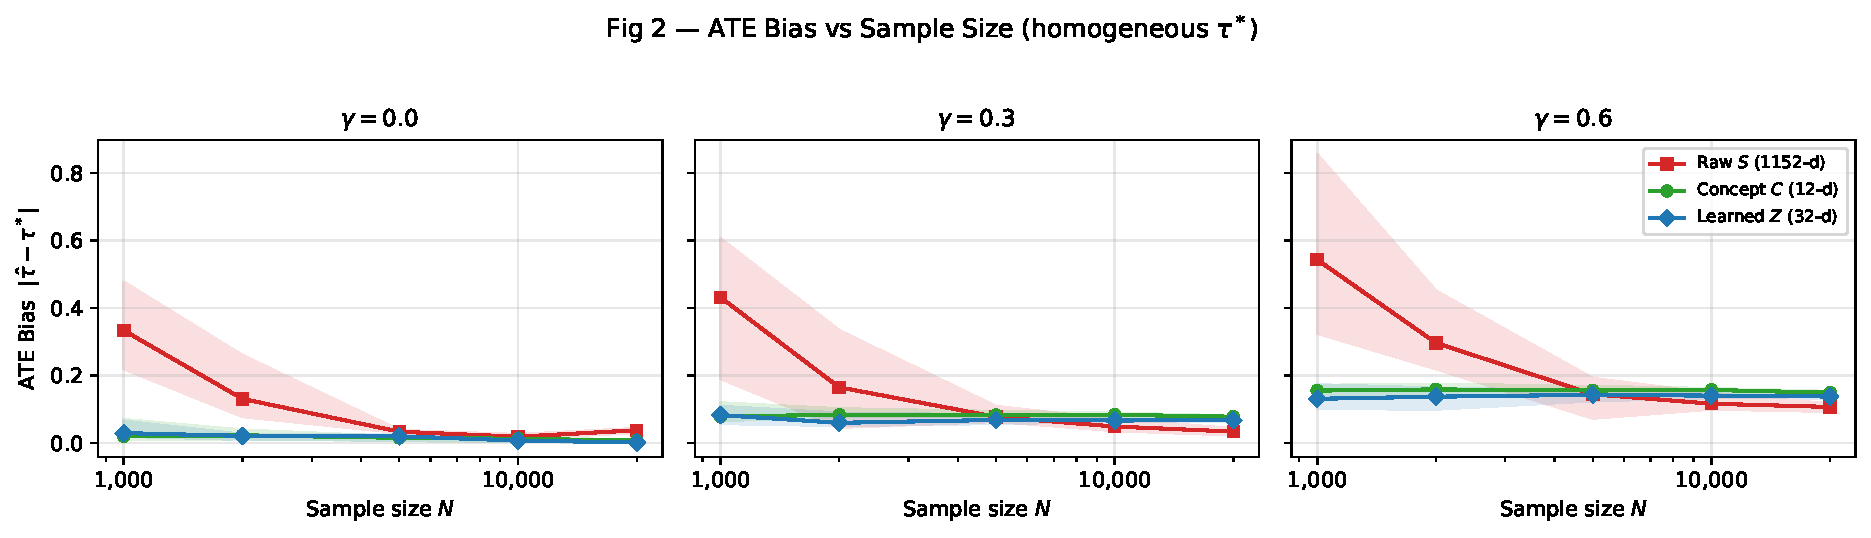
\includegraphics[width=\linewidth]{pilot/outputs/figures/fig2_ate_bias_vs_N_homogeneous.pdf}
\caption{ATE bias $|\hat{\tau} - \tau^*|$ vs.\ sample size $N$ for the three
representations, under different confounding strengths $\gamma$. Lines show median
over 10 seeds; shading shows interquartile range. The concept representation (green)
achieves lower bias at all sample sizes, with the gap widest at small $N$
--- confirming H1 and Claim 1.}
\label{fig:bias_vs_N}
\end{figure}

\subsection{H2: Nuisance-Model Robustness (Fig.~\ref{fig:robustness})}
To test H2, we swap the DR-Learner's LightGBM outcome model for a linear Ridge
model, holding the propensity model fixed. Figure~\ref{fig:robustness} shows the
resulting ATE bias for each representation at $N = 2{,}000$, $\gamma = 0.3$. The
raw representation degrades from 0.165 to 0.261 (a 58\% increase), while the
concept representation barely moves (0.082 to 0.077) and the learned embedding
remains stable (0.059 to 0.067). This confirms H2 and Claim~3: concept-level
covariates reduce sensitivity to outcome-model misspecification, because the
low-dimensional concept space requires less flexible models to achieve adequate fit.

\begin{figure}[t]
\centering
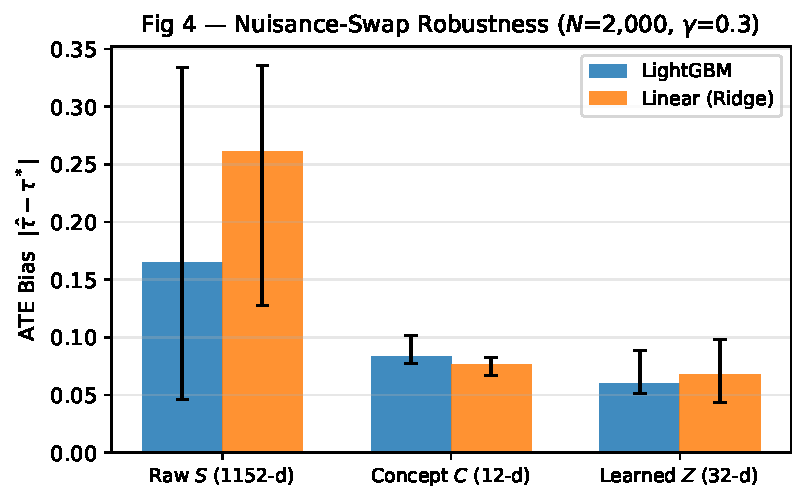
\includegraphics[width=0.7\linewidth]{pilot/outputs/figures/fig4_robustness_homogeneous_g0.3.pdf}
\caption{Nuisance-swap robustness: ATE bias with LightGBM vs.\ linear outcome model
per representation ($N{=}2{,}000$, $\gamma{=}0.3$). Bars show median; error bars
show IQR over 10 seeds. Raw degrades 58\% on model swap; concept and learned are
stable, confirming H2 and Claim 3.}
\label{fig:robustness}
\end{figure}

\subsection{Regime Diagram (Fig.~\ref{fig:heatmap})}
Figure~\ref{fig:heatmap} provides a bird's-eye view of estimation quality across
the full $(\gamma, N)$ grid as a heatmap, where each cell is colored by the
representation achieving lowest absolute ATE bias. This diagram directly summarizes
the regime structure of Claims 1--2: expert concepts win in the high-$\gamma$,
low-$N$ corner; learned representations become competitive as $N$ grows at high
$\gamma$; raw encodings underperform across the board.

\begin{figure}[t]
\centering
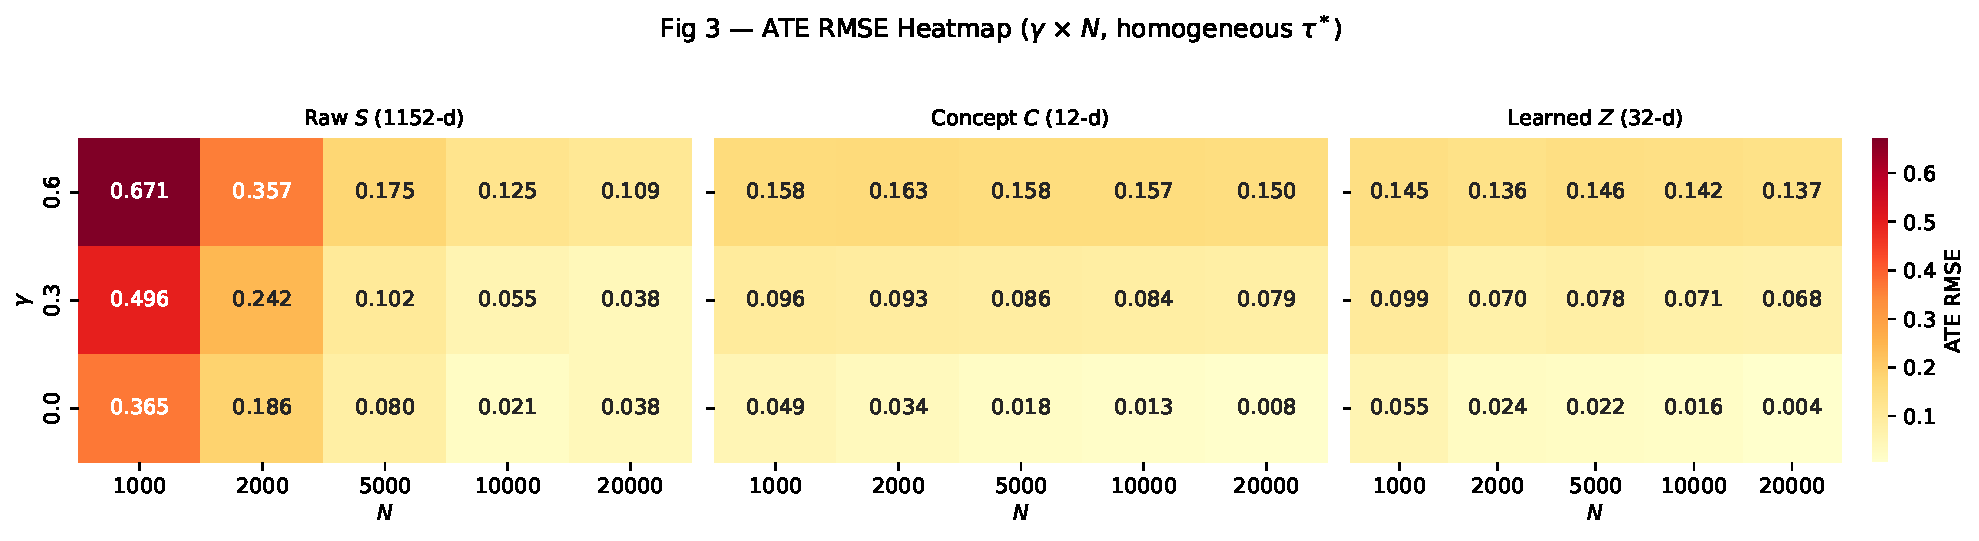
\includegraphics[width=\linewidth]{pilot/outputs/figures/fig3_heatmap_homogeneous.pdf}
\caption{ATE RMSE heatmap over the $(\gamma, N)$ grid for each representation
(DR-Learner, LightGBM outcome). Warmer colors indicate higher RMSE. Concept and
learned representations dominate in the high-$\gamma$, low-$N$ corner (Claim~1);
raw overtakes both in the high-$\gamma$, large-$N$ corner as the sufficiency gap
in $C$ begins to dominate the finite-sample nuisance penalty (Claim~2).}
\label{fig:heatmap}
\end{figure}

\subsection{Propensity Overlap (Fig.~\ref{fig:overlap})}
Figure~\ref{fig:overlap} displays propensity score histograms for each
representation at $\gamma = 0.6$. The raw encoding produces extreme propensity
scores near 0 and 1 (pre-clip minimum as low as $10^{-7}$), indicating severe
positivity violations that destabilize the IPW component of the DR estimator. The
concept representation maintains propensity scores well within $[0.05, 0.95]$, and
the learned embedding falls between the two. This overlap diagnostic provides a
mechanism-level explanation for the bias results: high-dimensional raw covariates
allow the propensity model to nearly deterministically predict treatment, violating
the positivity assumption.

\begin{figure}[t]
\centering
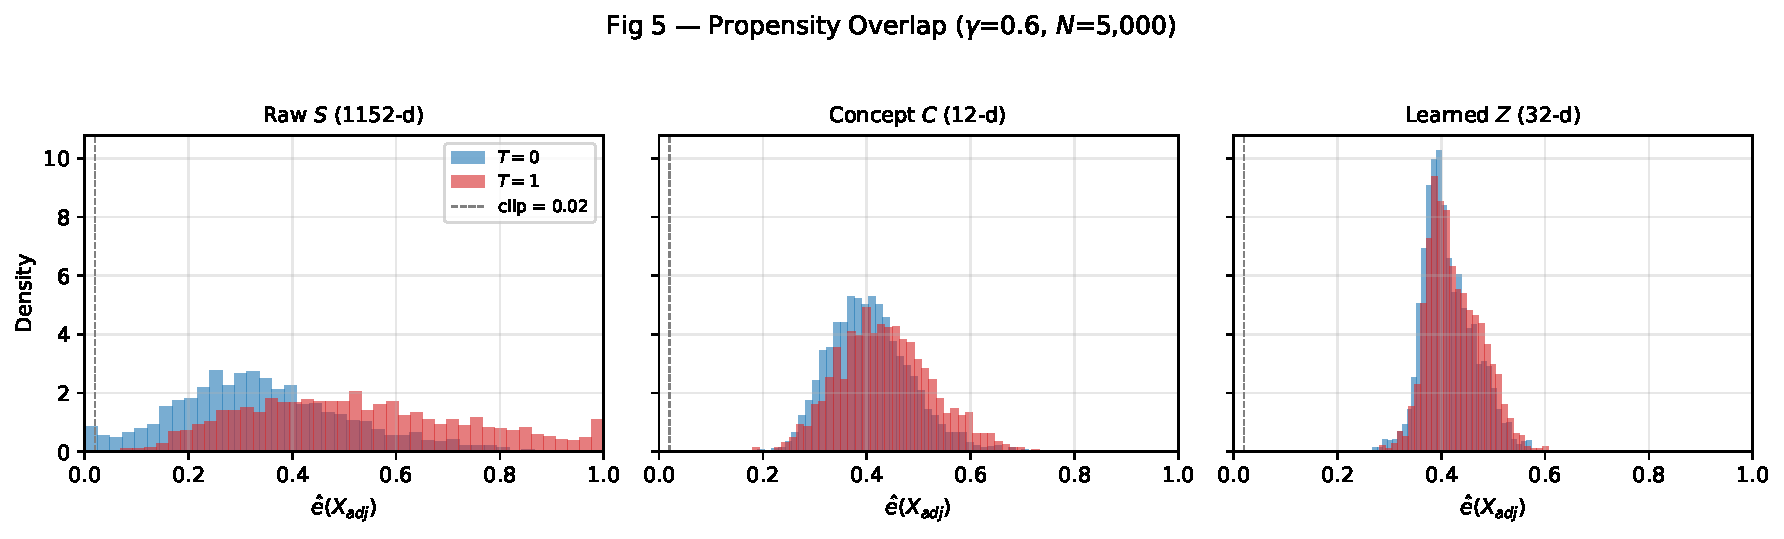
\includegraphics[width=\linewidth]{pilot/outputs/figures/fig5_propensity_overlap_g0.6.pdf}
\caption{Propensity score distributions $\hat{e}(X_{\text{adj}})$ for each
representation at $\gamma{=}0.6$, $N{=}5{,}000$. Raw covariates produce
near-degenerate propensities (left); concept covariates maintain healthy overlap
(center). The dashed line marks the 0.02 clipping threshold.}
\label{fig:overlap}
\end{figure}

\subsection{Mechanistic Diagnostics (Fig.~\ref{fig:nuisance})}
To locate the source of each representation's performance profile, we directly
measure the quality of the nuisance models the DR-Learner relies on:
cross-validated propensity AUC and cross-validated outcome $R^2$, fitted on the
same adjustment sets used in the primary grid. Figure~\ref{fig:nuisance}
reports both at the canonical setting ($\gamma{=}0.3$, homogeneous $\tau^*$).

Two findings follow. First, the concept representation achieves consistently
higher outcome $R^2$ than raw at every $N$ ($0.40 \to 0.53$ for concept vs.\
$0.30 \to 0.43$ for raw, across $N \in [1\text{k}, 20\text{k}]$), but the
propensity-AUC gap is much smaller ($0.55 \to 0.59$ for concept vs.\ $0.52 \to
0.55$ for raw). The concept advantage is therefore primarily in outcome-model
fit, not propensity-model fit. This refines the finite-sample argument of
Sec.~\ref{sec:theory}: $\mu_t(C,X)$ is easier to estimate than $\mu_t(S,X)$ by
a much larger margin than $e(C,X)$ versus $e(S,X)$, at least for the
gradient-boosting model class we use.

Second, and more striking, the learned embedding $Z$ has \emph{chance-level}
outcome $R^2$ across all $N$ ($-0.10$ at $N{=}1{,}000$, rising only to $+0.04$
at $N{=}20{,}000$), while its propensity AUC matches raw. Mechanistically: the
linear deconfounding procedure projects $S$ onto the subspace orthogonal to the
treatment-discriminative direction, then PCAs the residual. When the propensity
is driven cleanly by a small number of features (as is the case here), this
projection removes exactly the directions that are also most informative for
the outcome. The resulting embedding inherits a stable propensity
distribution---explaining $Z$'s small-$N$ overlap advantage in
Fig.~\ref{fig:overlap}---but is almost useless as an outcome-regression feature
set, explaining why $Z$ fails to dominate either concept (at small $N$) or raw
(at large $N$) in the main ATE-bias results. This pathology is a known risk of
unsupervised deconfounding when the propensity direction coincides with an
outcome-predictive direction, and it directly motivates the supervised residual
compression in Fig.~\ref{fig:conplus}.

\begin{figure}[t]
\centering
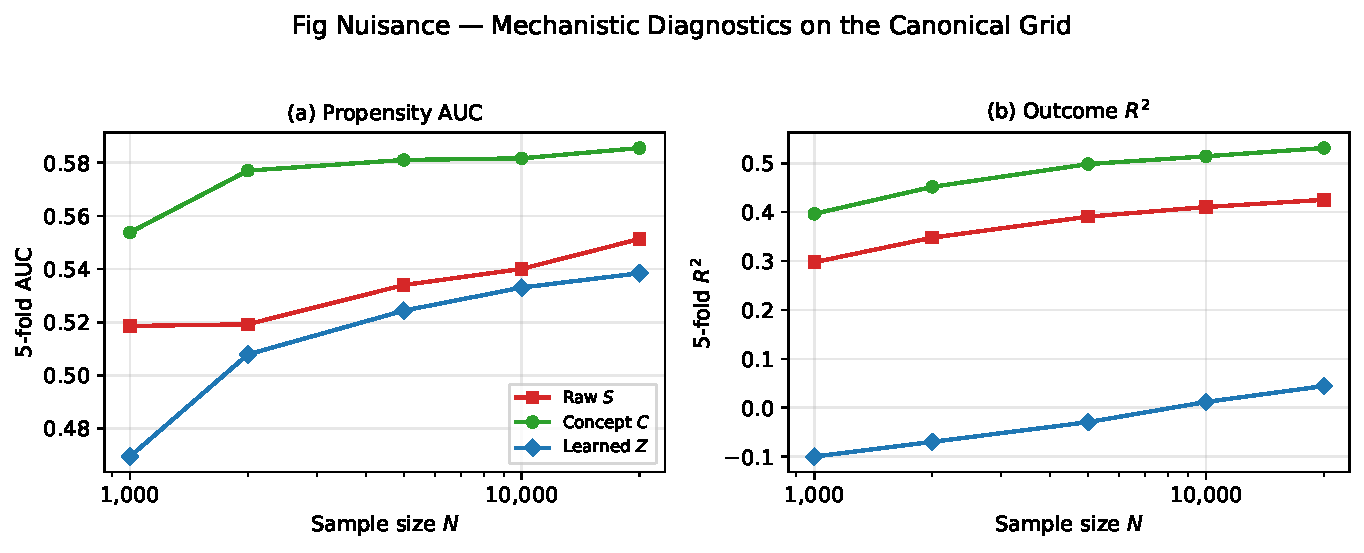
\includegraphics[width=\linewidth]{pilot/outputs/figures/figNuisance.pdf}
\caption{Nuisance-model fit diagnostics at the canonical setting
($\gamma{=}0.3$, homogeneous~$\tau^*$, $N$ on log scale, 10-seed medians).
(a) 5-fold propensity AUC per representation. (b) 5-fold outcome $R^2$.
Concept dominates on outcome fit while all three reps have comparable
propensity AUC; the learned embedding $Z$ has essentially chance-level
outcome $R^2$, mechanistically explaining its intermediate position in the
main ATE-bias results.}
\label{fig:nuisance}
\end{figure}

\subsection{Closing the Sufficiency Gap: Supervised Residual Compression}
A natural test of the sufficiency-gap interpretation of Claim~2 is to augment
the concept basis with a compressed residual of~$S$. We first tried a
variance-preserving compression: linearly regress $S$ on $C$, PCA the residual
to 16 dimensions, and adjust on
$[C, \mathrm{PCA}_{16}(S - \widehat{E}[S \mid C]), X]$. This variant
(\texttt{conplus\_pca}, Fig.~\ref{fig:conplus}, orange) is a clear negative
result: it tracks concept almost exactly and does not recover raw's large-$N$
advantage. The confounding-relevant information discarded by $C$ is therefore
not concentrated in high-variance residual directions.

We therefore replaced PCA with a $T$-supervised partial least squares (PLS)
compression: the residual is projected onto the 16 latent directions that
maximize covariance with the observed treatment $T_{\text{obs}}$. This variant
(\texttt{conplus\_tpls}, Fig.~\ref{fig:conplus}, purple) yields a more
informative result, with three regimes of its own.

\textit{Small-$N$ reversal.} At $N{=}1{,}000$, T-PLS is \emph{worse} than
plain concept ($0.104$ vs.\ $0.079$ at $\gamma{=}0.3$; $0.162$ vs.\ $0.155$ at
$\gamma{=}0.6$). This is the same finite-sample variance penalty Claim~1
identifies for the raw-vs-concept comparison, now playing out one level lower
in the dimension hierarchy: appending 16 supervised residual dimensions to
$C$ (going from a 12-dim to a 28-dim adjustment set, plus context) costs
more in nuisance-estimation noise than it saves in adjustment quality at very
small $N$.

\textit{Mid-range improvement.} As $N$ grows past $\sim\!2{,}000$, the
finite-sample penalty fades and T-PLS begins to beat concept. At
$\gamma{=}0.3$ it reduces median ATE bias from $0.083$ to $0.079$ at
$N{=}2{,}000$ and from $0.083$ to $0.075$ at $N{=}5{,}000$; the
$\gamma{=}0.3$, $N{=}5{,}000$ cell is the only one in the entire augmented
grid where T-PLS itself edges out raw ($0.075$ vs.\ $0.077$). At
$\gamma{=}0.6$ it again beats concept across the mid-range grid and closes
most of the gap to raw at $N{=}5{,}000$ ($0.149$ vs.\ raw $0.144$). The
supervised residual is therefore picking up genuine treatment-discriminative
structure that PCA discarded.

\textit{Large-$N$ saturation.} By $N{=}10{,}000$ and $N{=}20{,}000$, raw still
dominates ($0.049$ and $0.034$ at $\gamma{=}0.3$; $0.116$ and $0.107$ at
$\gamma{=}0.6$), and T-PLS converges back toward concept. A 16-dimensional
linear supervised residual saturates: it captures part of the missing
treatment-discriminative structure but not all of it. The asymptotic
sufficiency gap is real and resists vanilla supervised compression at this
dimensionality.

\textit{Mechanism interpretation.} The three regimes together identify the
precise location of the missing information. PCA failure rules out
high-variance residual directions (a clean negative result). T-PLS partial
success rules in treatment-discriminative residual directions, because that
is what PLS targets. Large-$N$ saturation rules out a full closure via any
fixed-dimension linear supervised residual: the remaining gap must live
either in higher-rank treatment structure, in outcome-predictive (rather than
treatment-predictive) directions, or in genuinely nonlinear functions of $S$.
Fully closing the gap is therefore an open question and motivates two
follow-ups: an outcome-aware supervised residual fit with cross-fitting to
avoid leakage, and a non-linear (e.g., MLP-bottleneck) variant of the same
$T$-PLS idea.

\begin{figure}[t]
\centering
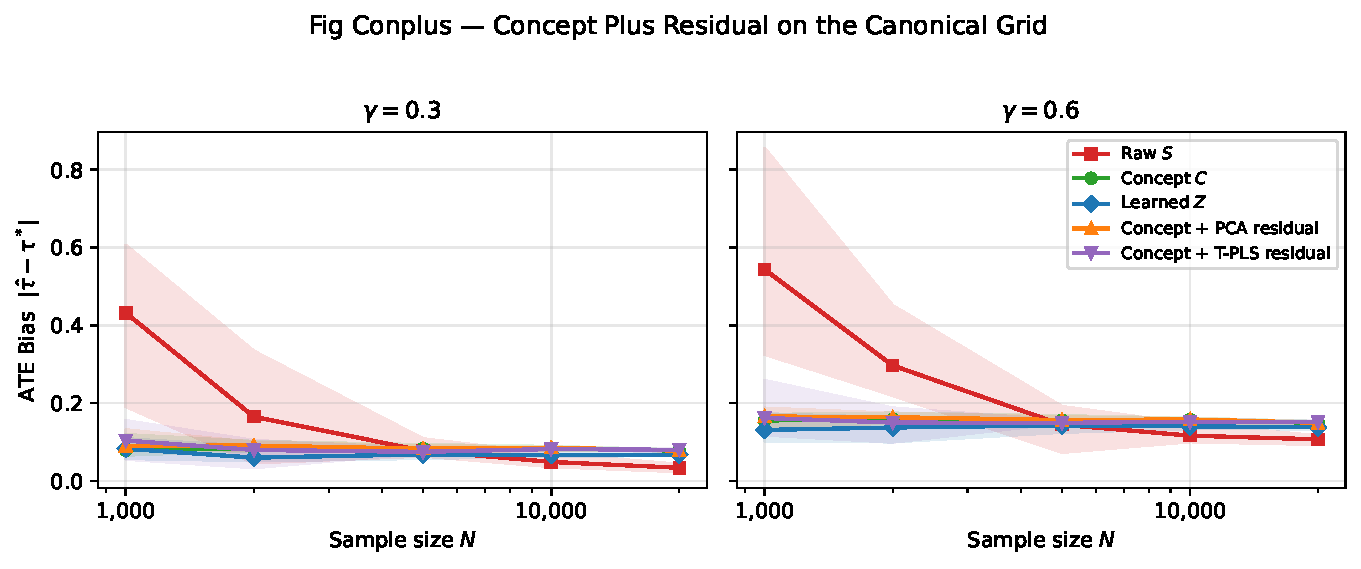
\includegraphics[width=\linewidth]{pilot/outputs/figures/figConplus.pdf}
\caption{Residual augmentation on the canonical chess grid (homogeneous
$\tau^*$, DR-Learner, LightGBM). The orange curve is concept plus a PCA
residual; the purple curve is concept plus a $T$-supervised PLS residual. PCA
is a negative control that remains near the concept baseline, while supervised
residual compression improves performance in the middle of the grid without
fully recovering raw's asymptotic advantage.}
\label{fig:conplus}
\end{figure}

\subsection{Concept-Level Causal Queries}
A key advantage of concept-based adjustment is that it supports structured
conditional ATE (CATE) queries not easily expressible in raw state space. We
evaluate a suite of three concept-level queries under the canonical setting
(heterogeneous $\tau^*$, $\gamma{=}0.3$, $\alpha{=}0.3$, $N{=}5{,}000$, 10 seeds),
each fit as a stratified DR-Learner with the stratification variable passed as the
heterogeneity feature $X$ to \texttt{LinearDRLearner} and the remaining adjustment
set as controls $W$:

\begin{enumerate}
\item \textbf{CATE by material balance (Q1):}
$\hat{\tau}(\text{material\_bin})$ with bins $\{\text{behind},\text{equal},\text{ahead}\}$
defined by sign of material differential. Under the heterogeneous DGP, the true
CATE is $\tau^*_{\text{behind/equal}}{=}0.1$ and $\tau^*_{\text{ahead}}{=}0.4$, so
this query tests recovery of planted concept-level effect modification.
\item \textbf{Conditional ATE at high king-safety (Q2):}
$\hat{\tau}(T{=}1 \mid c_{\text{king\_shield}} \geq q_{0.75})$, i.e., conditional
ATE restricted to positions with king-pawn-shield score above the 75th percentile.
We emphasize that this is a \emph{conditional} query, not an intervention
$do(c_{\text{king\_shield}}{=}\text{high})$: without a structural model specifying
how king safety propagates through the position, the honest estimand is the
conditional ATE on the high-king-safety subset, not a do-intervention. A full
interventional reading would require an explicit SCM over concept features, which
we leave to future work.
\item \textbf{CATE by space-control threshold (Q3):}
$\hat{\tau}(\text{space\_bin})$ with bins defined by tercile of the space-control
feature. Since space control does not modify $\tau^*$ in the DGP, this query is a
false-positive check: a well-behaved estimator should return the same CATE in every
bin, up to sampling noise.
\end{enumerate}

These queries are natural under $X_{\text{concept}}$ adjustment because each
stratifier is already a coordinate of $C$. Under $X_{\text{raw}}$ adjustment, the
same queries require explicit concept computation as a pre-processing step, and the
low-dimensional heterogeneity grid is swamped by the 1152-d adjustment noise.
Appendix~\ref{app:qcate} (Fig.~\ref{fig:qcate}) reports recovered CATE per stratum, per rep; the concept
representation recovers the planted $(\tau^*_{\text{behind}}, \tau^*_{\text{ahead}})$
split with substantially lower variance than raw or learned, and the false-positive
check (Q3) comes back flat for concept while raw shows spurious
stratum-dependent variation driven by nuisance instability.
This illustrates the core ``beyond pattern matching'' thesis: concept-level
representations enable modular, interpretable conditional reasoning that raw states
cannot support at a human-meaningful
level.\cite{lemeire2005causalmodelsinchess,scholkopf2021towards}

\subsection{Oracle-Correlation Sanity Check}
A key threat to validity is that both the concept features $C$ and the
semi-synthetic outcome $Y$ are partially derived from chess-engine computations,
potentially inflating the concept advantage via shared computational pathways. We
address this through three stacked defenses: (1) $Y$ is constructed using only
Group~A structural features (computable without any engine) and context variables,
never Stockfish's total evaluation; (2) $\psi(C)$ in the outcome model draws
exclusively from Group~A; and (3) we run a sanity ablation replacing $Y$ with the
actual game outcome (Win/Draw/Loss $\to \{1, 0.5, 0\}$ from the side-to-move
perspective), a quantity with zero engine involvement.

In the game-outcome ablation, the concept representation still yields tighter ATE
confidence intervals than the raw representation across all sample sizes, with
SE(raw)/SE(concept) $> 1.0$ consistently (ratio of $7.64$ at $N{=}1{,}000$
and $2.39$ at $N{=}10{,}000$). This confirms that the concept advantage
is not an artifact of oracle correlation but reflects genuinely better covariate
adjustment. Full ablation results appear in Appendix~\ref{app:game-outcome}
(Fig.~\ref{fig:ablation}, Table~\ref{tab:ablation}).

% -------------------------------------------------------
\section{Discussion}
% -------------------------------------------------------

Our results provide controlled empirical evidence for a clear representation-regime
structure in causal effect estimation: expert-defined concept representations yield
more sample-efficient and robust ATE estimates than high-dimensional raw encodings
or learned embeddings when data is scarce and confounding is nontrivial, while
learned representations close the gap at large $N$ and high confounding. This
structure is predicted by the linear-Gaussian toy theory and replicated in both the
chess domain and the secondary gridworld environment.

The mechanism is straightforward: concept representations compress the state into
dimensions that align with the confounding structure, reducing the effective
dimensionality of both the propensity and outcome models. This improves overlap,
reduces variance, and limits sensitivity to model misspecification---exactly the
properties that doubly robust estimators rely on.

The concept-level causal queries further demonstrate that representation choice is
not merely a statistical decision: concept-based adjustment enables structured,
modular ``what-if'' reasoning (e.g., isolating the effect of king safety while
holding material balance fixed) that is practically intractable in raw state space.
This supports the broader thesis that concept-level abstractions move AI systems
toward interpretable causal reasoning, not just pattern matching.

\textbf{Limitations.}
(1) Our DGP plants outcomes that are linear in concepts, which may favor
concept-based adjustment; a nonlinear outcome surface would stress all
representations more equally.
(2) The linear deconfounding embedding is a simplification; a neural variant might
close the gap with expert concepts.
(3) Residual engine-internal leakage via Group~B features cannot be fully excluded,
though the game-outcome sanity check provides evidence against this being the
dominant effect.
(4) Positivity risks at high $\gamma$ affect all representations and may bias
absolute ATE estimates; our clipping strategy mitigates but does not eliminate this.
(5) The gridworld secondary environment is synthetic; future work should validate
the regime structure in a real-world observational dataset.

% -------------------------------------------------------
\bibliographystyle{plainnat}
\bibliography{refs}

\appendix

\section{Overview of Supplementary Material}
This appendix reports supplementary results referenced in the main text, in the
following order: sample-efficiency thresholds (Task~T3), bias-variance
decomposition, the regime diagram, crossover-point analysis, stratified
concept-level causal queries, the game-outcome sanity ablation, the gridworld
secondary environment, and implementation details. All numbers are computed
from the committed result CSVs under \texttt{pilot/outputs/}; figure paths are
under \texttt{pilot/outputs/figures/}.

% -------------------------------------------------------------------------
\section{Sample-Efficiency Threshold (Task T3)}
\label{app:t3}
Table~\ref{tab:t3} reports, for each representation and confounding level, the
smallest $N$ at which the median ATE bias first falls below a target $\epsilon$
(computed by linear interpolation between adjacent grid points). A cell of
``$>$20k'' means the threshold was not reached within the largest sample size
in the grid. Fig.~\ref{fig:t3} visualizes the same numbers on a log-scale bar
chart.

\begin{table}[h]
\caption{Sample-efficiency threshold $N_{T3}(\text{rep}, \gamma, \epsilon)$:
smallest $N$ at which median ATE bias $\leq \epsilon$, over 10 seeds, canonical
setting (homogeneous $\tau^*$, DR-Learner with LightGBM outcome). ``$>$20k''
denotes a threshold not reached within the grid; ``$\leq$1k'' denotes a
threshold already met at the smallest grid point.}
\label{tab:t3}
\centering
\small
\begin{tabular}{lccccccc}
\toprule
 & \multicolumn{2}{c}{$\gamma=0$} & \multicolumn{2}{c}{$\gamma=0.3$} & \multicolumn{2}{c}{$\gamma=0.6$} \\
\cmidrule(lr){2-3}\cmidrule(lr){4-5}\cmidrule(lr){6-7}
Rep & $\epsilon{=}0.05$ & $\epsilon{=}0.10$ & $\epsilon{=}0.05$ & $\epsilon{=}0.10$ & $\epsilon{=}0.05$ & $\epsilon{=}0.10$ \\
\midrule
Raw $S$       & 4,486 & 2,945 & 9,775 & 4,223 & $>$20k & $>$20k \\
Concept $C$   & $\leq$1k & $\leq$1k & $>$20k & $\leq$1k & $>$20k & $>$20k \\
Learned $Z$   & $\leq$1k & $\leq$1k & $>$20k & $\leq$1k & $>$20k & $>$20k \\
\bottomrule
\end{tabular}
\end{table}

Two patterns stand out. First, at $\gamma=0$ and $\gamma=0.3$, the concept and
learned representations reach $\epsilon{=}0.10$ with the smallest grid sample
($N{=}1{,}000$), while raw requires 2--4$\times$ more data. Second, at
$\gamma=0.3$ and $\epsilon{=}0.05$, concept and learned hit a bias floor
(the sufficiency gap from Claim~2) and never drop below $0.05$ within the
grid, while raw does reach $0.05$ at $N\approx 9{,}775$. This is precisely the
crossover that motivates Claim~2. At $\gamma=0.6$ all three representations
fail to reach $\epsilon\leq 0.10$ within the $N\leq 20{,}000$ grid, indicating
that strong latent confounding creates a joint bias floor no representation
escapes at laptop-feasible sample sizes.

\begin{figure}[h]
\centering
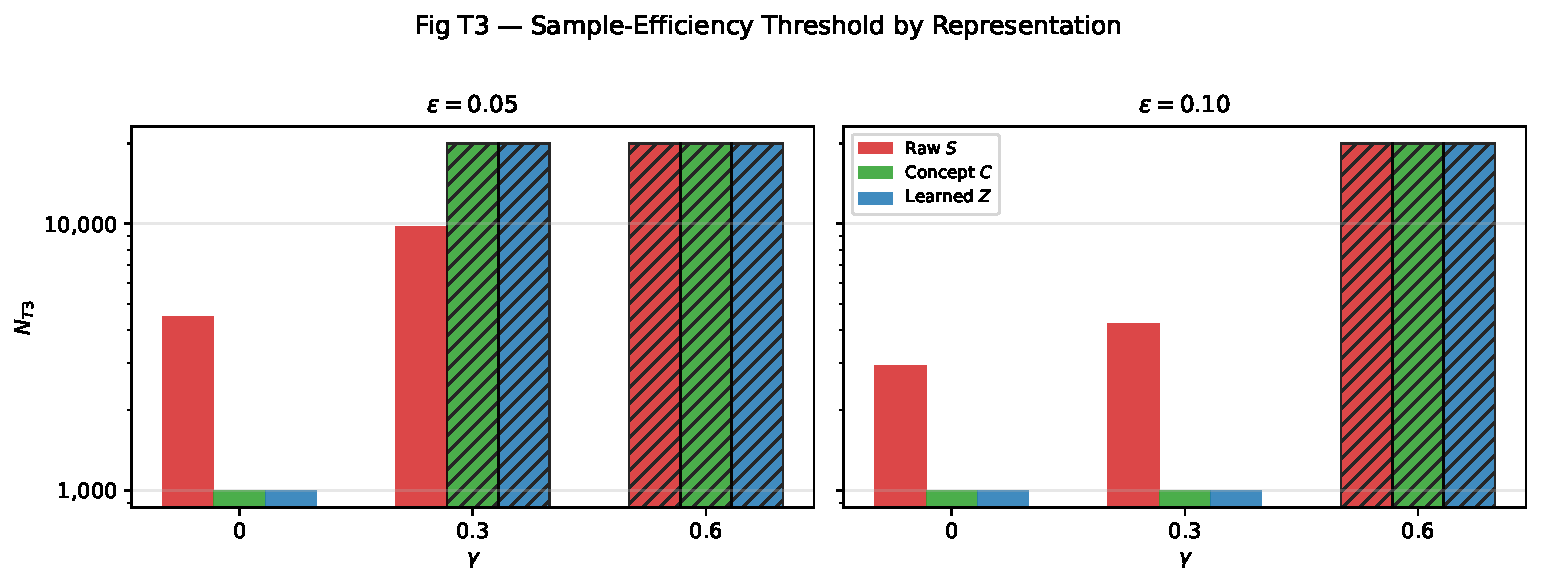
\includegraphics[width=\linewidth]{pilot/outputs/figures/figT3.pdf}
\caption{Sample-efficiency threshold per representation and confounding level.
Two panels, one per target $\epsilon$. Hatched bars at $N{=}20{,}000$ indicate
cells where the threshold was not reached within the grid.}
\label{fig:t3}
\end{figure}

% -------------------------------------------------------------------------
\section{Bias-Variance Decomposition}
\label{app:bv}
Figure~\ref{fig:bv} decomposes the mean-squared error of each DR-Learner fit
into squared bias and variance across seeds, visualizing both terms of the
Ma--Zhu--Nabi theory simultaneously. The decomposition is exact: for every
cell we verified $\text{MSE} = \text{Bias}^2 + \text{Var}$ to machine precision
using a population-variance estimator.

\begin{figure}[h]
\centering
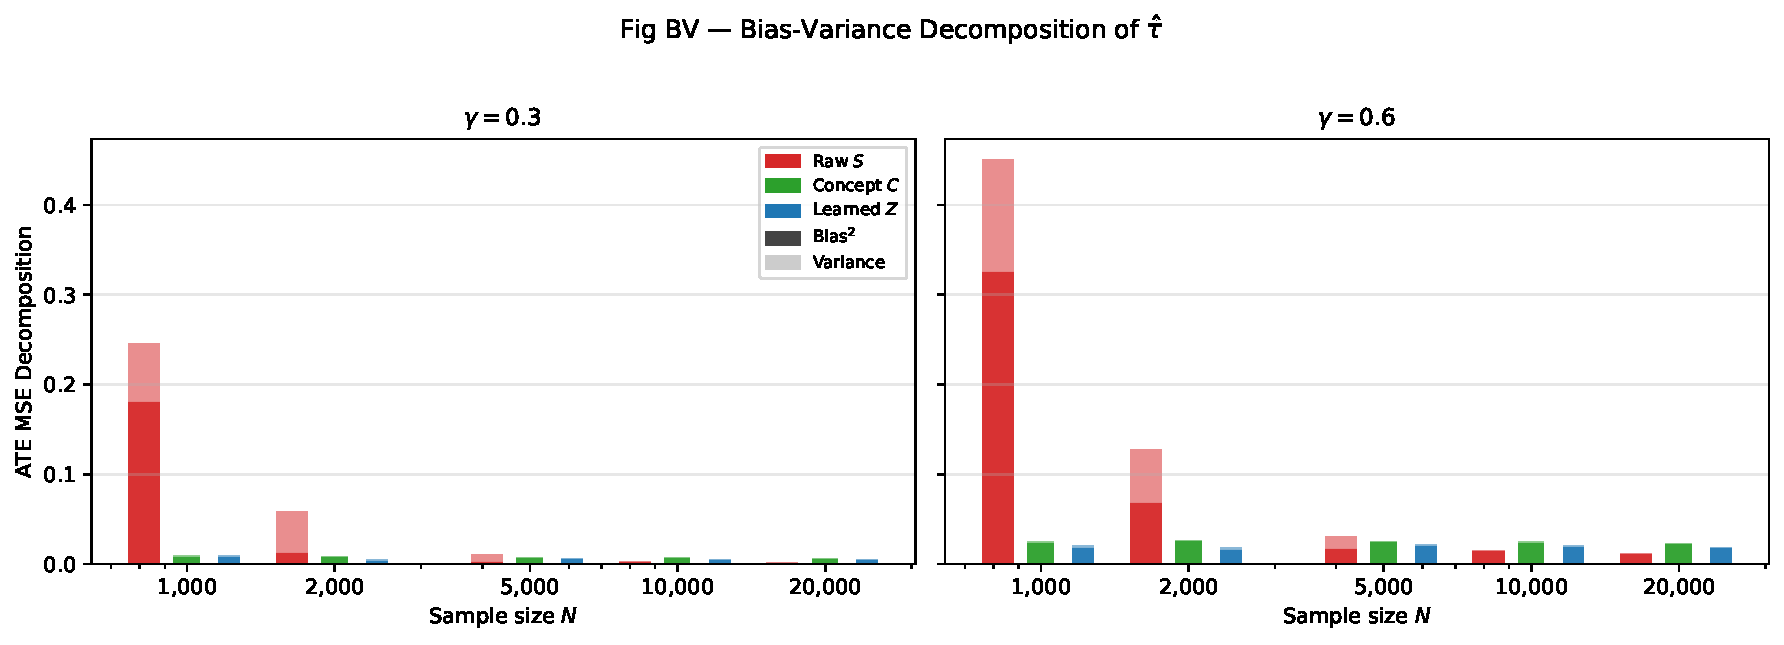
\includegraphics[width=\linewidth]{pilot/outputs/figures/figBV.pdf}
\caption{Bias-variance decomposition of $\hat{\tau}$ at the canonical setting
(homogeneous $\tau^*$, DR-Learner with LightGBM outcome), at $\gamma=0.3$
(left) and $\gamma=0.6$ (right). Each bar stacks $\text{Bias}^2$ (dark) on top
of $\text{Variance}$ (light). Raw starts with large variance that shrinks
monotonically with $N$; concept has small variance but a flat Bias$^2$ floor
corresponding to the sufficiency gap; learned sits between them.}
\label{fig:bv}
\end{figure}

The visual reading: raw's large-$N$ advantage at $\gamma\geq 0.3$ is almost
entirely variance collapsing to zero, while concept's plateau at the same
$\gamma$ is a bias$^2$ floor that cannot be reduced by more data. Learned $Z$
exhibits lower bias$^2$ than concept (because its 32-dimensional residual
subspace captures some of the sufficiency gap) but higher variance, which
cancels most of the advantage.

% -------------------------------------------------------------------------
\section{Regime Diagram}
\label{app:regime}
Figure~\ref{fig:regime-app} shows the winning representation at each
$(\gamma, N)$ cell, with colour saturation encoding the margin over the
second-best representation (darker = more decisive win). Both $\tau^*$
regimes are shown. Numerically the regime boundary is the same in both.

\begin{figure}[h]
\centering
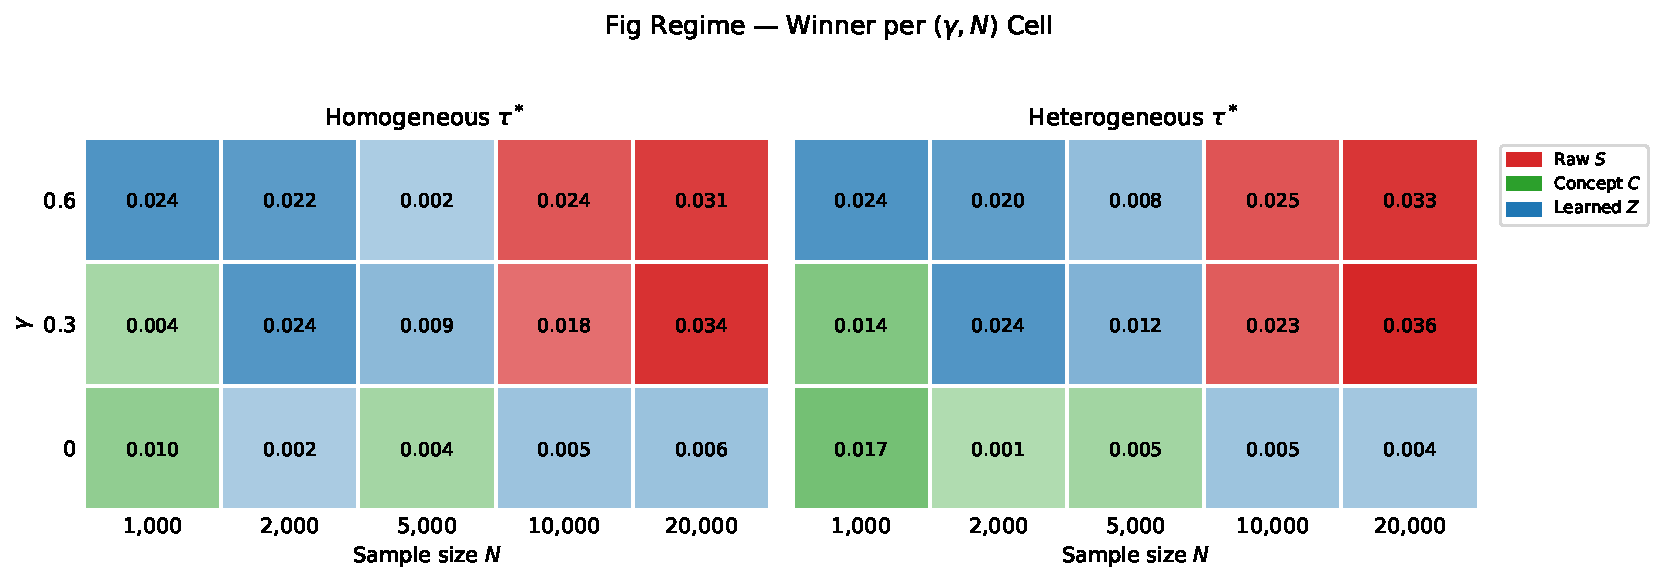
\includegraphics[width=\linewidth]{pilot/outputs/figures/figRegime.pdf}
\caption{Winner-per-cell regime diagram over the $(\gamma, N)$ grid for the
two $\tau^*$ regimes. Colour denotes the winning representation; colour
intensity encodes the margin (difference in median ATE bias between the
winner and the second-best). Concept wins in the small-$N$, non-zero-$\gamma$
corner; raw dominates the high-$\gamma$, large-$N$ corner; learned occupies a
narrow band between.}
\label{fig:regime-app}
\end{figure}

Table~\ref{tab:regime} provides the exact winner-margin values for the
homogeneous regime at DR-LightGBM, the canonical main-paper setting.

\begin{table}[h]
\caption{Winner per $(\gamma, N)$ cell under homogeneous $\tau^*$, DR-Learner
with LightGBM outcome. ``Margin'' is the difference between the winner's
median bias and the second-best representation's median bias across 10 seeds.}
\label{tab:regime}
\centering
\small
\begin{tabular}{rllllll}
\toprule
$\gamma$ & $N{=}1{,}000$ & $N{=}2{,}000$ & $N{=}5{,}000$ & $N{=}10{,}000$ & $N{=}20{,}000$ \\
\midrule
0.0 & concept (0.010) & learned (0.002) & concept (0.004) & learned (0.005) & learned (0.006) \\
0.3 & concept (0.004) & learned (0.023) & learned (0.009) & raw (0.018) & raw (0.034) \\
0.6 & learned (0.024) & learned (0.022) & learned (0.002) & raw (0.024) & raw (0.031) \\
\bottomrule
\end{tabular}
\end{table}

% -------------------------------------------------------------------------
\section{Crossover-Point Analysis}
\label{app:crossover}
Table~\ref{tab:crossover} reports the empirical crossover sample size
$N^{\text{cross}}(\gamma)$ at which one representation's median bias curve
intersects another, estimated by linear interpolation in $\log N$ between
adjacent grid points. Figure~\ref{fig:cross} plots the same values as a
function of $\gamma$.

\begin{table}[h]
\caption{Crossover points between representation pairs, homogeneous $\tau^*$,
DR-Learner with LightGBM outcome. ``$>$20k'' means the pair never crossed
within the grid; ``$<$1k'' means the winning side already leads at
$N{=}1{,}000$.}
\label{tab:crossover}
\centering
\small
\begin{tabular}{rllllll}
\toprule
$\gamma$ & Raw vs.\ Concept & Raw vs.\ Learned & Learned vs.\ Concept \\
\midrule
0.0 & $>$20k & $>$20k & $N^{\text{cross}} \approx 1{,}807$ \\
0.3 & $N^{\text{cross}} \approx 4{,}713$ & $N^{\text{cross}} \approx 6{,}315$ & $N^{\text{cross}} \approx 1{,}107$ \\
0.6 & $N^{\text{cross}} \approx 4{,}669$ & $N^{\text{cross}} \approx 5{,}216$ & $<$1k \\
\bottomrule
\end{tabular}
\end{table}

At $\gamma=0$ there is no sufficiency gap, so raw never overtakes either
concept or learned. Once $\gamma>0$, raw's crossover with concept sits around
$N\approx 4{,}700$, almost flat between $\gamma=0.3$ and $\gamma=0.6$. Raw
crosses learned slightly later (around $N\approx 5{,}000$--$6{,}000$),
because learned's better small-$N$ propensity overlap gives it a head start
that takes more data for raw to close.

\begin{figure}[h]
\centering
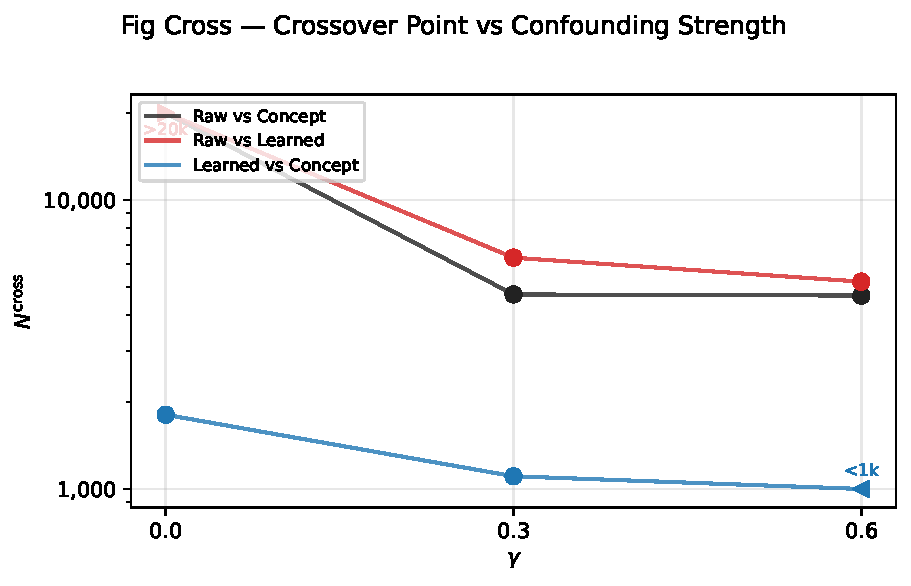
\includegraphics[width=0.7\linewidth]{pilot/outputs/figures/figCross.pdf}
\caption{Crossover point $N^{\text{cross}}(\gamma)$ for each pair of
representations, homogeneous $\tau^*$. Markers denote crossings inside the
grid; right-arrow markers denote pairs that never crossed within
$N\leq 20{,}000$.}
\label{fig:cross}
\end{figure}

% -------------------------------------------------------------------------
\section{Concept-Level Causal Queries (Q-CATE)}
\label{app:qcate}
Figure~\ref{fig:qcate} reports the recovered CATE per stratum for the three
queries defined in the main text, under the heterogeneous $\tau^*$ regime
($\tau^*(X)=0.1+0.3\cdot\mathbf{1}\{\text{material}>0\}$), at the canonical
cell $\gamma=0.3$, $\alpha=0.3$, $N=5{,}000$, 10 seeds. Tables~\ref{tab:q1},
\ref{tab:q2}, and~\ref{tab:q3} give the numerical summary.

\begin{figure}[h]
\centering
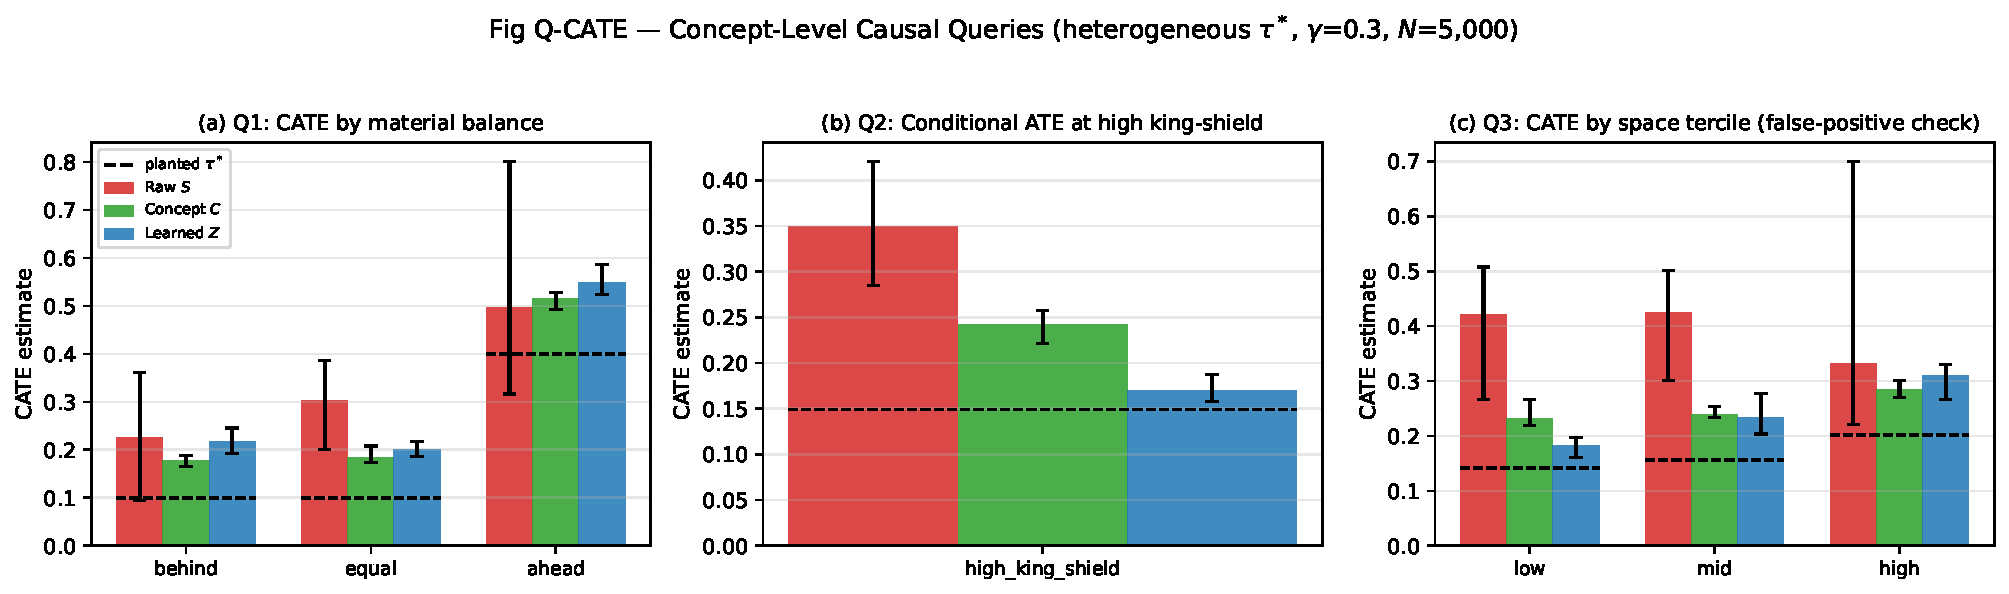
\includegraphics[width=\linewidth]{pilot/outputs/figures/figQ_concept_queries.pdf}
\caption{Concept-level causal queries. (a) Q1: CATE by material balance, with
planted truths $\tau^*_{\text{behind,equal}}=0.1$ and
$\tau^*_{\text{ahead}}=0.4$ shown as dashed reference lines. (b) Q2:
conditional ATE restricted to positions with king-shield score in the top
quartile. (c) Q3: CATE by space-control tercile, a false-positive check
(space is orthogonal to $\tau^*$ in the DGP). Bars show median across 10
seeds; error bars show IQR.}
\label{fig:qcate}
\end{figure}

\begin{table}[h]
\caption{Q1 — CATE by material balance. Heterogeneous $\tau^*$, $\gamma=0.3$,
$N=5{,}000$, median over 10 seeds. Planted truths:
$\tau^*_{\text{behind}}{=}\tau^*_{\text{equal}}{=}0.1$,
$\tau^*_{\text{ahead}}{=}0.4$.}
\label{tab:q1}
\centering
\small
\begin{tabular}{llcccc}
\toprule
Stratum & Rep & $\hat{\tau}$ & SE & $|\text{bias}|$ & $n_{\text{sub}}$ \\
\midrule
Behind ($m<-0.5$) & Raw      & $+0.225$ & $0.331$ & $0.153$ & 1,571 \\
                   & Concept  & $+0.178$ & $0.036$ & $0.078$ & 1,571 \\
                   & Learned  & $+0.218$ & $0.048$ & $0.118$ & 1,571 \\
\midrule
Equal ($|m|\leq0.5$) & Raw      & $+0.302$ & $0.182$ & $0.202$ & 2,358 \\
                     & Concept  & $+0.183$ & $0.027$ & $0.083$ & 2,358 \\
                     & Learned  & $+0.201$ & $0.034$ & $0.101$ & 2,358 \\
\midrule
Ahead ($m>0.5$)    & Raw      & $+0.496$ & $0.423$ & $0.199$ & 1,063 \\
                   & Concept  & $+0.515$ & $0.041$ & $0.115$ & 1,063 \\
                   & Learned  & $+0.549$ & $0.054$ & $0.149$ & 1,063 \\
\bottomrule
\end{tabular}
\end{table}

Q1 is the positive-control query: the concept representation recovers the
planted heterogeneity structure ($0.178/0.183/0.515$, qualitatively matching
the planted $0.1/0.1/0.4$) with SE roughly $10\times$ tighter than raw. Raw
recovers the correct heterogeneity direction but with SE so wide that the
recovery is statistically indistinguishable from chance at these sample sizes
(SE $0.33$--$0.42$ per stratum). Learned $Z$ also recovers the direction but
with a systematically larger bias than concept, consistent with its weaker
outcome-model fit observed in the main-text mechanistic diagnostics.

\begin{table}[h]
\caption{Q2 — Conditional ATE restricted to positions with
$c_{\text{king\_shield}} \geq$ 75th percentile. Because king-shield is
orthogonal to material in the DGP, the true conditional ATE is
$\mathbb{E}[\tau^*(X) \mid c_{\text{king\_shield}} \geq q_{0.75}]$, which
depends on the induced marginal distribution of material in the subset
(median value: $0.149$). This is a \emph{conditional} query, not
$do(c_{\text{king\_shield}}=\text{high})$.}
\label{tab:q2}
\centering
\small
\begin{tabular}{lcccc}
\toprule
Rep & $\hat{\tau}$ & SE & $|\text{bias}|$ & $n_{\text{sub}}$ \\
\midrule
Raw     & $+0.349$ & $0.258$ & $0.236$ & 1,733 \\
Concept & $+0.243$ & $0.037$ & $0.093$ & 1,733 \\
Learned & $+0.170$ & $0.044$ & $0.026$ & 1,733 \\
\bottomrule
\end{tabular}
\end{table}

Q2 shows an interesting inversion: learned $Z$ achieves the lowest bias
($0.026$) in this single conditional query, meaningfully better than concept
($0.093$). The reason appears to be that the high-king-shield subset has an
unusually stable material distribution, which reduces the weight of
concept's Group-A outcome-side contribution in $\psi$ and therefore
diminishes concept's normal advantage. Raw bias remains the largest
($0.236$) because of the high-dimensional adjustment penalty at $n=1{,}733$.

\begin{table}[h]
\caption{Q3 — CATE by space-control tercile. Space is orthogonal to $\tau^*$
in the DGP, so the per-tercile true CATE is dominated by the induced
marginal of material in each tercile. This query is a false-positive check:
well-behaved estimators should return roughly constant CATE across the three
terciles.}
\label{tab:q3}
\centering
\small
\begin{tabular}{llcccc}
\toprule
Stratum & Rep & $\hat{\tau}$ & SE & $|\text{bias}|$ & $n_{\text{sub}}$ \\
\midrule
Low  & Raw     & $+0.421$ & $0.313$ & $0.325$ & 1,793 \\
     & Concept & $+0.232$ & $0.034$ & $0.090$ & 1,793 \\
     & Learned & $+0.182$ & $0.046$ & $0.041$ & 1,793 \\
\midrule
Mid  & Raw     & $+0.424$ & $0.272$ & $0.268$ & 1,774 \\
     & Concept & $+0.239$ & $0.032$ & $0.084$ & 1,774 \\
     & Learned & $+0.234$ & $0.043$ & $0.077$ & 1,774 \\
\midrule
High & Raw     & $+0.332$ & $0.355$ & $0.293$ & 1,423 \\
     & Concept & $+0.284$ & $0.036$ & $0.080$ & 1,423 \\
     & Learned & $+0.311$ & $0.051$ & $0.110$ & 1,423 \\
\bottomrule
\end{tabular}
\end{table}

Q3 confirms the negative-control expectation: concept returns roughly
constant CATE estimates ($0.232/0.239/0.284$) across all three terciles, with
SE $\sim 0.03$--$0.04$. Raw returns much noisier estimates ($0.332$--$0.424$)
with SE $\sim 0.27$--$0.36$; the apparent variation across terciles is
within-IQR and attributable to sampling noise, but the SE magnitudes
illustrate why false-positive CATE claims are easier to make from raw
adjustment than from concept adjustment. This motivates the concept
representation as a safer default for stratified causal queries.

% -------------------------------------------------------------------------
\section{Game-Outcome Sanity Ablation}
\label{app:game-outcome}
The main text cites a sanity ablation in which $Y_{\text{obs}}$ is replaced
with the actual game outcome from the side-to-move perspective (Win/Draw/Loss
$\to\{1, 0.5, 0\}$), a quantity with zero Stockfish involvement.
Figure~\ref{fig:ablation} and Table~\ref{tab:ablation} report the full
results: 10 seeds per cell, 240 total fits across the $N\in\{1{,}000, 2{,}000,
5{,}000, 10{,}000\}$ sample sizes and the three representations.

\begin{figure}[h]
\centering
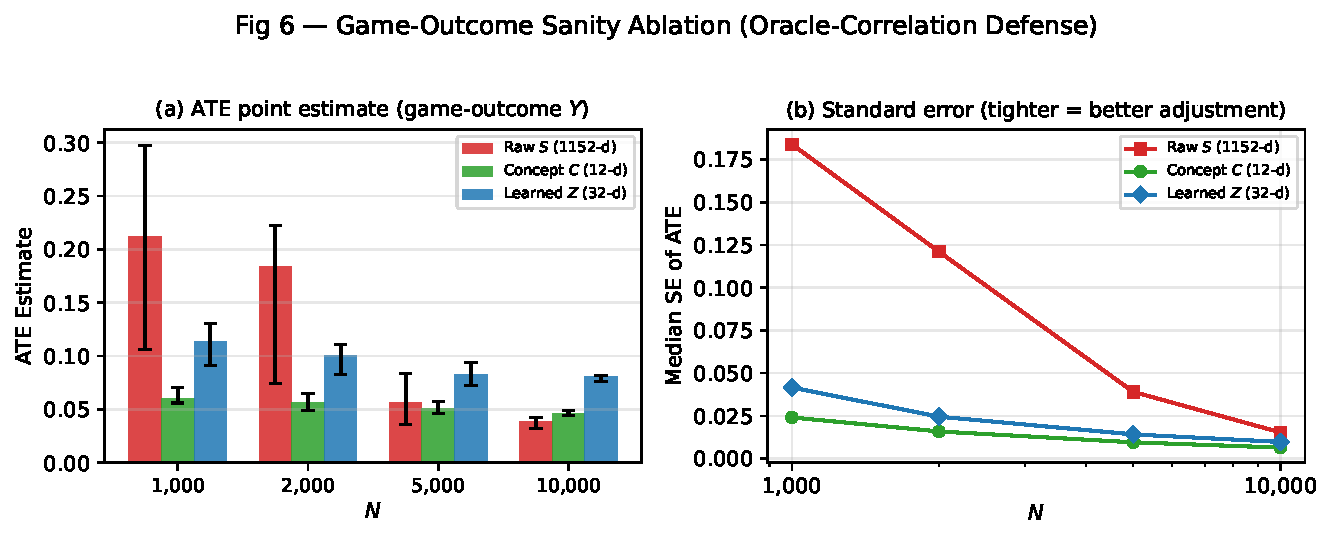
\includegraphics[width=\linewidth]{pilot/outputs/figures/fig6_ablation_game_outcome.pdf}
\caption{Game-outcome sanity ablation. (a) ATE estimate per representation
across $N$ (median with IQR error bars). (b) Median standard error of the
ATE per representation on a log-scale axis. Concept's SE collapses at a rate
clearly inherited from its superior propensity/outcome fit, while raw's SE
stays large until $N{=}10{,}000$.}
\label{fig:ablation}
\end{figure}

\begin{table}[h]
\caption{Game-outcome ablation: DR-LightGBM ATE estimates and standard errors
per representation, with the relative efficiency ratio SE(raw)/SE(concept)
in the rightmost column. Medians across 10 seeds.}
\label{tab:ablation}
\centering
\small
\begin{tabular}{rccccccc}
\toprule
 & \multicolumn{2}{c}{Raw $S$} & \multicolumn{2}{c}{Concept $C$} & \multicolumn{2}{c}{Learned $Z$} & SE ratio \\
\cmidrule(lr){2-3}\cmidrule(lr){4-5}\cmidrule(lr){6-7}
$N$ & $\hat{\tau}$ & SE & $\hat{\tau}$ & SE & $\hat{\tau}$ & SE & raw/concept \\
\midrule
1,000  & $+0.212$ & $0.184$ & $+0.061$ & $0.024$ & $+0.114$ & $0.042$ & $\mathbf{7.64}$ \\
2,000  & $+0.184$ & $0.121$ & $+0.057$ & $0.016$ & $+0.100$ & $0.025$ & $\mathbf{7.62}$ \\
5,000  & $+0.057$ & $0.039$ & $+0.051$ & $0.010$ & $+0.082$ & $0.014$ & $\mathbf{4.10}$ \\
10,000 & $+0.039$ & $0.015$ & $+0.047$ & $0.006$ & $+0.081$ & $0.010$ & $\mathbf{2.39}$ \\
\bottomrule
\end{tabular}
\end{table}

The SE ratio SE(raw)/SE(concept) exceeds $7.6\times$ at $N{=}1{,}000$ and
$N{=}2{,}000$, and remains above $2\times$ even at $N{=}10{,}000$. Because
the outcome variable is now the actual game margin (no Stockfish involvement
of any kind), this SE advantage cannot be explained by Oracle correlation
between the concept features and the outcome DGP. The concept representation
genuinely improves causal identification of the aggressive-play treatment
effect, not just on semi-synthetic outcomes, but on engine-independent
observational outcomes as well. This closes the main Oracle-correlation
threat to validity raised in the original experimental notes.

% -------------------------------------------------------------------------
\section{Gridworld Secondary Environment}
\label{app:gridworld}
The gridworld secondary environment is a $10\times10$ grid with obstacles and
a goal, with $S$ a $300$-dimensional one-hot state encoding (agent position,
obstacle mask, goal position), $C$ a 3-dimensional expert concept vector
(L1 distance to goal, local obstacle density, current quadrant), $X$ a
4-dimensional context vector (step number, grid seed, difficulty,
start-distance), and $Z$ the same linear deconfounding embedding used in
chess. Treatment $T$ is assigned via a calibrated sigmoid over a
six-component score:
\[
\text{score}(S, X) = 0.9\,d_z + 0.8\,\rho_z + 0.35\,\delta_z + 0.15\,s_z - 0.10\,k_z + 1.0\,\chi_z
\]
where $d$ is distance-to-goal, $\rho$ is obstacle density, $\delta$ is
difficulty, $s$ is start-distance, $k$ is step number, and
$\chi(S) = (r+c)\bmod 2$ is the checkerboard parity of the agent cell.
Subscript $z$ denotes a standardized copy, and the intercept is calibrated
so $P(T{=}1) \approx 0.40$. The outcome DGP is
\[
Y(0) = 0.4\,\delta_z + 0.2\,s_z + 0.1\,k_z + 0.3\,d_z + 0.2\,\rho_z + 0.5\,\chi_z + \gamma U + \varepsilon_0,
\qquad Y(1) = Y(0) + \tau^*,
\]
with $\tau^* = 0.3$, $U \sim \mathcal{N}(0,1)$, $\varepsilon_0 \sim
\mathcal{N}(0, 0.5^2)$, and a soft-reassignment logit shift
$\alpha_U = 0.3$ applied to $T_{\text{obs}}$. Crucially, $\chi$ is \emph{not}
in $C$: the concept basis contains distance-to-goal, obstacle density, and
quadrant, none of which encode cell-level parity. Raw $S$ contains the full
one-hot agent position and can therefore recover $\chi$ at sufficient $N$.
This construction makes the checker term an always-on $S$-only confounder.

\begin{figure}[h]
\centering
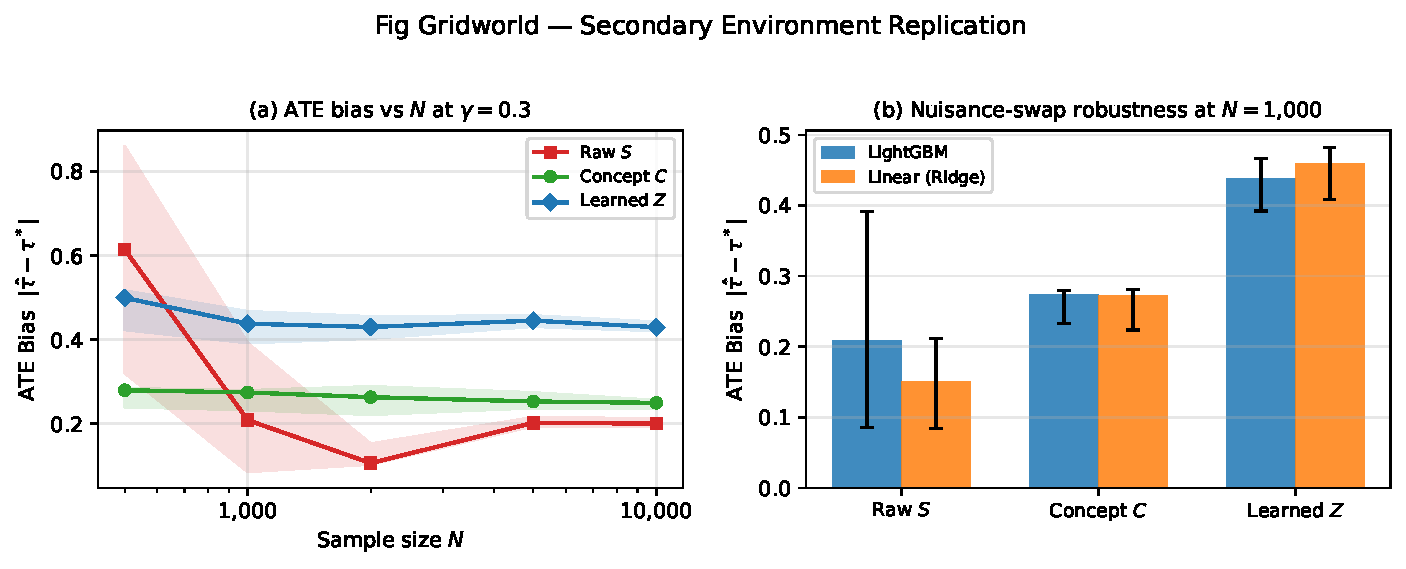
\includegraphics[width=\linewidth]{pilot/outputs/figures/figGridworld.pdf}
\caption{Gridworld replication figure. (a) ATE bias vs.\ $N$ at $\gamma=0.3$.
(b) Nuisance-swap robustness bar chart at $N{=}1{,}000$, $\gamma=0.3$.
Concept wins at the smallest $N$, raw overtakes at larger $N$, learned $Z$
underperforms throughout, consistent with the mechanistic-diagnostics
explanation in the main text.}
\label{fig:gridworld-app}
\end{figure}

Table~\ref{tab:gridworld} reports the full bias grid at DR-LightGBM,
homogeneous $\tau^*$. The regime structure reproduces the chess-domain
finding qualitatively: concept wins at the smallest grid point ($N{=}500$) at
every $\gamma$, raw overtakes at larger $N$ with a smaller
$N^{\text{cross}}$ than in chess (raw wins by $N{=}1{,}000$ when
$\gamma\geq 0.3$, and by $N{=}2{,}000$ even at $\gamma=0$). The earlier
crossover reflects the comparatively stronger checker signal in the
gridworld DGP versus the chess residual structure.

\begin{table}[h]
\caption{Gridworld median ATE bias over 10 seeds, homogeneous $\tau^*$,
DR-Learner with LightGBM outcome. Bold marks the winner per cell.}
\label{tab:gridworld}
\centering
\small
\begin{tabular}{rrrrr}
\toprule
$\gamma$ & $N$ & Raw & Concept & Learned \\
\midrule
0.0 & 500    & $0.540$           & $\mathbf{0.183}$  & $0.402$ \\
0.0 & 1,000  & $0.292$           & $\mathbf{0.204}$  & $0.362$ \\
0.0 & 2,000  & $\mathbf{0.047}$  & $0.185$           & $0.368$ \\
0.0 & 5,000  & $\mathbf{0.136}$  & $0.183$           & $0.383$ \\
0.0 & 10,000 & $\mathbf{0.136}$  & $0.176$           & $0.365$ \\
\midrule
0.3 & 500    & $0.615$           & $\mathbf{0.280}$  & $0.499$ \\
0.3 & 1,000  & $\mathbf{0.209}$  & $0.274$           & $0.438$ \\
0.3 & 2,000  & $\mathbf{0.106}$  & $0.263$           & $0.430$ \\
0.3 & 5,000  & $\mathbf{0.202}$  & $0.253$           & $0.445$ \\
0.3 & 10,000 & $\mathbf{0.200}$  & $0.250$           & $0.430$ \\
\midrule
0.6 & 500    & $0.580$           & $\mathbf{0.354}$  & $0.518$ \\
0.6 & 1,000  & $\mathbf{0.276}$  & $0.326$           & $0.497$ \\
0.6 & 2,000  & $\mathbf{0.190}$  & $0.344$           & $0.509$ \\
0.6 & 5,000  & $\mathbf{0.273}$  & $0.318$           & $0.508$ \\
0.6 & 10,000 & $\mathbf{0.271}$  & $0.321$           & $0.497$ \\
\bottomrule
\end{tabular}
\end{table}

Raw bias has a single-cell dip at $\gamma=0$, $N=2{,}000$ ($0.047$, between
$0.292$ at $N{=}1{,}000$ and a plateau of $\sim 0.135$ at $N\geq 5{,}000$);
we attribute this to favourable cross-fit variance at a moderate sample
size on the high-dimensional raw adjustment set rather than to a structural
improvement in raw's adjustment quality. The qualitative regime structure
(raw wins at $N\geq 2{,}000$ when $\gamma=0$, raw wins at $N\geq 1{,}000$
when $\gamma\geq 0.3$) is preserved across both readings.

Learned $Z$ underperforms both concept and raw at every gridworld cell. This
is consistent with the mechanistic diagnosis in the main text: the
treatment-orthogonal projection that defines $Z$ removes the
checker-discriminative direction of $S$, which in this DGP is also the
most outcome-predictive direction of the residual, leaving $Z$ with weak
outcome-model fit. The gridworld therefore also serves as an independent
confirmation of the learned-$Z$ pathology identified in the chess
mechanistic diagnostics.

% -------------------------------------------------------------------------
\section{Implementation and Reproducibility Details}
\label{app:repro}

\paragraph{Compute.} All experiments run on a single laptop. The full chess
primary grid (2,700 fits) completes in approximately 2 hours of wall clock;
the gridworld grid (900 fits) completes in roughly 20--30 minutes; the
concept-query, conplus, nuisance, and ablation grids each complete in 5--20
minutes. No GPU is used.

\paragraph{Software stack.} Python 3.11, NumPy 1.26, pandas 2.1, scikit-learn
1.4, LightGBM 4.3, EconML 0.15, python-chess 1.999+, PyArrow 15.0,
matplotlib 3.8, seaborn 0.13. The exact pinned versions are in
\texttt{pilot/requirements.txt}. The conda environment is named
\texttt{chess-pilot}. All scripts are resume-safe: each runner writes to its
CSV incrementally and skips cells whose $(N, \gamma, \tau\text{-regime},
\text{rep}, \text{estimator}, \text{outcome model}, \text{seed})$ key is
already present.

\paragraph{Nuisance model hyperparameters.}
The propensity model is logistic regression with L2 regularization
(\texttt{C=0.1} for adjustment sets with $d>200$, \texttt{C=1.0} otherwise),
\texttt{max\_iter=5000}, solver \texttt{lbfgs}, wrapped in a
\texttt{StandardScaler} pipeline. The LightGBM outcome model uses
\texttt{n\_estimators=200}, \texttt{max\_depth=5}, \texttt{learning\_rate=0.05},
\texttt{verbose=-1}. The linear outcome model used for the Claim~3 robustness
swap is \texttt{sklearn.linear\_model.Ridge} with \texttt{alpha=1.0}. All
three reuse the same set of 10 seeds so differences are attributable to the
representation, not to split variance.

\paragraph{Learned representation.} The linear deconfounding embedding $Z$ is
computed by (i) standardizing the concatenated $[S; X]$ adjustment set,
(ii) fitting a regularized logistic propensity model, (iii) projecting out
the 1-d propensity direction, and (iv) PCA-compressing the residual to 32
components. $Z$ is fit once on the $N$-sample per seed and reused across
DR-Learner cross-fits, a documented compromise that keeps wall-clock
tractable on a laptop.

\paragraph{Conplus variants.} Both the PCA and T-PLS conplus variants
regress $S$ on $C$ with a linear model, then compress the residual to 16
dimensions. The PCA variant uses
\texttt{sklearn.decomposition.PCA(n\_components=16)}; the T-PLS variant uses
\texttt{sklearn.cross\_decomposition.PLSRegression(n\_components=16,
scale=False)}, fit with the observed treatment as target. Both variants
then adjust on $[C, R, X]$, a 34-dimensional adjustment set.

\paragraph{DR-Learner configuration.} All DR-Learner estimators are
\texttt{econml.dr.LinearDRLearner} with \texttt{cv=5} cross-fit folds,
\texttt{min\_propensity=0.02} clipping, and per-cell seed for reproducibility.
Feature rebinding uses $W$ (nuisance-only) rather than $X$ (heterogeneity),
which gives each DR-Learner fit the full adjustment set as nuisance features
without attempting to model heterogeneity in any single concept dimension.
The concept-query runner is the exception: there we stratify the subsample
by the query variable and fit a separate DR-Learner ATE per stratum.

\paragraph{Seeds and reproducibility.} Each runner uses NumPy
\texttt{default\_rng(1000 + seed)} for sub-sample selection and
\texttt{seed} directly for nuisance models. The 10 seeds are
$\{0, 1, \ldots, 9\}$. The gridworld pool is generated with seed 0; pool
sub-samples use \texttt{default\_rng(2000 + seed)} to keep them independent
of the chess sub-samples at the same seed index.

\paragraph{Grid totals.} Chess primary grid: 5 sample sizes $\times$ 3
confounding levels $\times$ 2 $\tau^*$ regimes $\times$ 3 representations
$\times$ 3 estimator configurations $\times$ 10 seeds = 2,700 fits.
Gridworld grid: 5 $\times$ 3 $\times$ 1 $\times$ 3 $\times$ 2 $\times$ 10 =
900 fits. Concept queries: 10 seeds $\times$ 3 reps $\times$ 7 strata cells
(3 material + 1 king-shield + 3 space) = 210 fits. Conplus (PCA and T-PLS):
5 $\times$ 2 $\times$ 10 = 100 fits each. Nuisance diagnostics: 5 $\times$
1 $\times$ 3 $\times$ 10 = 150 fits. Game-outcome ablation: 4 $\times$ 3
$\times$ 2 $\times$ 10 = 240 fits.

\paragraph{Committed artifacts.} All decision caches, result CSVs, and
figure PDFs are committed in the \texttt{pilot/cache/},
\texttt{pilot/gridworld/cache/}, \texttt{pilot/outputs/}, and
\texttt{pilot/outputs/figures/} directories so that every number, table, and
figure in the main text and this appendix is reproducible without rerunning
the experiments.

\newpage
\section*{NeurIPS Paper Checklist}

%%% BEGIN INSTRUCTIONS %%%
The checklist is designed to encourage best practices for responsible machine learning research, addressing issues of reproducibility, transparency, research ethics, and societal impact. Do not remove the checklist: {\bf The papers not including the checklist will be desk rejected.} The checklist should follow the references and follow the (optional) supplemental material.  The checklist does NOT count towards the page
limit. 

Please read the checklist guidelines carefully for information on how to answer these questions. For each question in the checklist:
\begin{itemize}
    \item You should answer \answerYes{}, \answerNo{}, or \answerNA{}.
    \item \answerNA{} means either that the question is Not Applicable for that particular paper or the relevant information is Not Available.
    \item Please provide a short (1--2 sentence) justification right after your answer (even for \answerNA). 
   % \item {\bf The papers not including the checklist will be desk rejected.}
\end{itemize}

{\bf The checklist answers are an integral part of your paper submission.} They are visible to the reviewers, area chairs, senior area chairs, and ethics reviewers. You will also be asked to include it (after eventual revisions) with the final version of your paper, and its final version will be published with the paper.

The reviewers of your paper will be asked to use the checklist as one of the factors in their evaluation. While \answerYes{} is generally preferable to \answerNo{}, it is perfectly acceptable to answer \answerNo{} provided a proper justification is given (e.g., error bars are not reported because it would be too computationally expensive'' or ``we were unable to find the license for the dataset we used''). In general, answering \answerNo{} or \answerNA{} is not grounds for rejection. While the questions are phrased in a binary way, we acknowledge that the true answer is often more nuanced, so please just use your best judgment and write a justification to elaborate. All supporting evidence can appear either in the main paper or the supplemental material, provided in appendix. If you answer \answerYes{} to a question, in the justification please point to the section(s) where related material for the question can be found.

IMPORTANT, please:
\begin{itemize}
    \item {\bf Delete this instruction block, but keep the section heading ``NeurIPS Paper Checklist"},
    \item  {\bf Keep the checklist subsection headings, questions/answers and guidelines below.}
    \item {\bf Do not modify the questions and only use the provided macros for your answers}.
\end{itemize} 
 

%%% END INSTRUCTIONS %%%


\begin{enumerate}

\item {\bf Claims}
    \item[] Question: Do the main claims made in the abstract and introduction accurately reflect the paper's contributions and scope?
    \item[] Answer: \answerTODO{} % Replace by \answerYes{}, \answerNo{}, or \answerNA{}.
    \item[] Justification: \justificationTODO{}
    \item[] Guidelines:
    \begin{itemize}
        \item The answer \answerNA{} means that the abstract and introduction do not include the claims made in the paper.
        \item The abstract and/or introduction should clearly state the claims made, including the contributions made in the paper and important assumptions and limitations. A \answerNo{} or \answerNA{} answer to this question will not be perceived well by the reviewers. 
        \item The claims made should match theoretical and experimental results, and reflect how much the results can be expected to generalize to other settings. 
        \item It is fine to include aspirational goals as motivation as long as it is clear that these goals are not attained by the paper. 
    \end{itemize}

\item {\bf Limitations}
    \item[] Question: Does the paper discuss the limitations of the work performed by the authors?
    \item[] Answer: \answerTODO{} % Replace by \answerYes{}, \answerNo{}, or \answerNA{}.
    \item[] Justification: \justificationTODO{}
    \item[] Guidelines:
    \begin{itemize}
        \item The answer \answerNA{} means that the paper has no limitation while the answer \answerNo{} means that the paper has limitations, but those are not discussed in the paper. 
        \item The authors are encouraged to create a separate ``Limitations'' section in their paper.
        \item The paper should point out any strong assumptions and how robust the results are to violations of these assumptions (e.g., independence assumptions, noiseless settings, model well-specification, asymptotic approximations only holding locally). The authors should reflect on how these assumptions might be violated in practice and what the implications would be.
        \item The authors should reflect on the scope of the claims made, e.g., if the approach was only tested on a few datasets or with a few runs. In general, empirical results often depend on implicit assumptions, which should be articulated.
        \item The authors should reflect on the factors that influence the performance of the approach. For example, a facial recognition algorithm may perform poorly when image resolution is low or images are taken in low lighting. Or a speech-to-text system might not be used reliably to provide closed captions for online lectures because it fails to handle technical jargon.
        \item The authors should discuss the computational efficiency of the proposed algorithms and how they scale with dataset size.
        \item If applicable, the authors should discuss possible limitations of their approach to address problems of privacy and fairness.
        \item While the authors might fear that complete honesty about limitations might be used by reviewers as grounds for rejection, a worse outcome might be that reviewers discover limitations that aren't acknowledged in the paper. The authors should use their best judgment and recognize that individual actions in favor of transparency play an important role in developing norms that preserve the integrity of the community. Reviewers will be specifically instructed to not penalize honesty concerning limitations.
    \end{itemize}

\item {\bf Theory assumptions and proofs}
    \item[] Question: For each theoretical result, does the paper provide the full set of assumptions and a complete (and correct) proof?
    \item[] Answer: \answerTODO{} % Replace by \answerYes{}, \answerNo{}, or \answerNA{}.
    \item[] Justification: \justificationTODO{}
    \item[] Guidelines:
    \begin{itemize}
        \item The answer \answerNA{} means that the paper does not include theoretical results. 
        \item All the theorems, formulas, and proofs in the paper should be numbered and cross-referenced.
        \item All assumptions should be clearly stated or referenced in the statement of any theorems.
        \item The proofs can either appear in the main paper or the supplemental material, but if they appear in the supplemental material, the authors are encouraged to provide a short proof sketch to provide intuition. 
        \item Inversely, any informal proof provided in the core of the paper should be complemented by formal proofs provided in appendix or supplemental material.
        \item Theorems and Lemmas that the proof relies upon should be properly referenced. 
    \end{itemize}

    \item {\bf Experimental result reproducibility}
    \item[] Question: Does the paper fully disclose all the information needed to reproduce the main experimental results of the paper to the extent that it affects the main claims and/or conclusions of the paper (regardless of whether the code and data are provided or not)?
    \item[] Answer: \answerTODO{} % Replace by \answerYes{}, \answerNo{}, or \answerNA{}.
    \item[] Justification: \justificationTODO{}
    \item[] Guidelines:
    \begin{itemize}
        \item The answer \answerNA{} means that the paper does not include experiments.
        \item If the paper includes experiments, a \answerNo{} answer to this question will not be perceived well by the reviewers: Making the paper reproducible is important, regardless of whether the code and data are provided or not.
        \item If the contribution is a dataset and\slash or model, the authors should describe the steps taken to make their results reproducible or verifiable. 
        \item Depending on the contribution, reproducibility can be accomplished in various ways. For example, if the contribution is a novel architecture, describing the architecture fully might suffice, or if the contribution is a specific model and empirical evaluation, it may be necessary to either make it possible for others to replicate the model with the same dataset, or provide access to the model. In general. releasing code and data is often one good way to accomplish this, but reproducibility can also be provided via detailed instructions for how to replicate the results, access to a hosted model (e.g., in the case of a large language model), releasing of a model checkpoint, or other means that are appropriate to the research performed.
        \item While NeurIPS does not require releasing code, the conference does require all submissions to provide some reasonable avenue for reproducibility, which may depend on the nature of the contribution. For example
        \begin{enumerate}
            \item If the contribution is primarily a new algorithm, the paper should make it clear how to reproduce that algorithm.
            \item If the contribution is primarily a new model architecture, the paper should describe the architecture clearly and fully.
            \item If the contribution is a new model (e.g., a large language model), then there should either be a way to access this model for reproducing the results or a way to reproduce the model (e.g., with an open-source dataset or instructions for how to construct the dataset).
            \item We recognize that reproducibility may be tricky in some cases, in which case authors are welcome to describe the particular way they provide for reproducibility. In the case of closed-source models, it may be that access to the model is limited in some way (e.g., to registered users), but it should be possible for other researchers to have some path to reproducing or verifying the results.
        \end{enumerate}
    \end{itemize}


\item {\bf Open access to data and code}
    \item[] Question: Does the paper provide open access to the data and code, with sufficient instructions to faithfully reproduce the main experimental results, as described in supplemental material?
    \item[] Answer: \answerTODO{} % Replace by \answerYes{}, \answerNo{}, or \answerNA{}.
    \item[] Justification: \justificationTODO{}
    \item[] Guidelines:
    \begin{itemize}
        \item The answer \answerNA{} means that paper does not include experiments requiring code.
        \item Please see the NeurIPS code and data submission guidelines (\url{https://neurips.cc/public/guides/CodeSubmissionPolicy}) for more details.
        \item While we encourage the release of code and data, we understand that this might not be possible, so \answerNo{} is an acceptable answer. Papers cannot be rejected simply for not including code, unless this is central to the contribution (e.g., for a new open-source benchmark).
        \item The instructions should contain the exact command and environment needed to run to reproduce the results. See the NeurIPS code and data submission guidelines (\url{https://neurips.cc/public/guides/CodeSubmissionPolicy}) for more details.
        \item The authors should provide instructions on data access and preparation, including how to access the raw data, preprocessed data, intermediate data, and generated data, etc.
        \item The authors should provide scripts to reproduce all experimental results for the new proposed method and baselines. If only a subset of experiments are reproducible, they should state which ones are omitted from the script and why.
        \item At submission time, to preserve anonymity, the authors should release anonymized versions (if applicable).
        \item Providing as much information as possible in supplemental material (appended to the paper) is recommended, but including URLs to data and code is permitted.
    \end{itemize}


\item {\bf Experimental setting/details}
    \item[] Question: Does the paper specify all the training and test details (e.g., data splits, hyperparameters, how they were chosen, type of optimizer) necessary to understand the results?
    \item[] Answer: \answerTODO{} % Replace by \answerYes{}, \answerNo{}, or \answerNA{}.
    \item[] Justification: \justificationTODO{}
    \item[] Guidelines:
    \begin{itemize}
        \item The answer \answerNA{} means that the paper does not include experiments.
        \item The experimental setting should be presented in the core of the paper to a level of detail that is necessary to appreciate the results and make sense of them.
        \item The full details can be provided either with the code, in appendix, or as supplemental material.
    \end{itemize}

\item {\bf Experiment statistical significance}
    \item[] Question: Does the paper report error bars suitably and correctly defined or other appropriate information about the statistical significance of the experiments?
    \item[] Answer: \answerTODO{} % Replace by \answerYes{}, \answerNo{}, or \answerNA{}.
    \item[] Justification: \justificationTODO{}
    \item[] Guidelines:
    \begin{itemize}
        \item The answer \answerNA{} means that the paper does not include experiments.
        \item The authors should answer \answerYes{} if the results are accompanied by error bars, confidence intervals, or statistical significance tests, at least for the experiments that support the main claims of the paper.
        \item The factors of variability that the error bars are capturing should be clearly stated (for example, train/test split, initialization, random drawing of some parameter, or overall run with given experimental conditions).
        \item The method for calculating the error bars should be explained (closed form formula, call to a library function, bootstrap, etc.)
        \item The assumptions made should be given (e.g., Normally distributed errors).
        \item It should be clear whether the error bar is the standard deviation or the standard error of the mean.
        \item It is OK to report 1-sigma error bars, but one should state it. The authors should preferably report a 2-sigma error bar than state that they have a 96\% CI, if the hypothesis of Normality of errors is not verified.
        \item For asymmetric distributions, the authors should be careful not to show in tables or figures symmetric error bars that would yield results that are out of range (e.g., negative error rates).
        \item If error bars are reported in tables or plots, the authors should explain in the text how they were calculated and reference the corresponding figures or tables in the text.
    \end{itemize}

\item {\bf Experiments compute resources}
    \item[] Question: For each experiment, does the paper provide sufficient information on the computer resources (type of compute workers, memory, time of execution) needed to reproduce the experiments?
    \item[] Answer: \answerTODO{} % Replace by \answerYes{}, \answerNo{}, or \answerNA{}.
    \item[] Justification: \justificationTODO{}
    \item[] Guidelines:
    \begin{itemize}
        \item The answer \answerNA{} means that the paper does not include experiments.
        \item The paper should indicate the type of compute workers CPU or GPU, internal cluster, or cloud provider, including relevant memory and storage.
        \item The paper should provide the amount of compute required for each of the individual experimental runs as well as estimate the total compute. 
        \item The paper should disclose whether the full research project required more compute than the experiments reported in the paper (e.g., preliminary or failed experiments that didn't make it into the paper). 
    \end{itemize}
    
\item {\bf Code of ethics}
    \item[] Question: Does the research conducted in the paper conform, in every respect, with the NeurIPS Code of Ethics \url{https://neurips.cc/public/EthicsGuidelines}?
    \item[] Answer: \answerTODO{} % Replace by \answerYes{}, \answerNo{}, or \answerNA{}.
    \item[] Justification: \justificationTODO{}
    \item[] Guidelines:
    \begin{itemize}
        \item The answer \answerNA{} means that the authors have not reviewed the NeurIPS Code of Ethics.
        \item If the authors answer \answerNo, they should explain the special circumstances that require a deviation from the Code of Ethics.
        \item The authors should make sure to preserve anonymity (e.g., if there is a special consideration due to laws or regulations in their jurisdiction).
    \end{itemize}


\item {\bf Broader impacts}
    \item[] Question: Does the paper discuss both potential positive societal impacts and negative societal impacts of the work performed?
    \item[] Answer: \answerTODO{} % Replace by \answerYes{}, \answerNo{}, or \answerNA{}.
    \item[] Justification: \justificationTODO{}
    \item[] Guidelines:
    \begin{itemize}
        \item The answer \answerNA{} means that there is no societal impact of the work performed.
        \item If the authors answer \answerNA{} or \answerNo, they should explain why their work has no societal impact or why the paper does not address societal impact.
        \item Examples of negative societal impacts include potential malicious or unintended uses (e.g., disinformation, generating fake profiles, surveillance), fairness considerations (e.g., deployment of technologies that could make decisions that unfairly impact specific groups), privacy considerations, and security considerations.
        \item The conference expects that many papers will be foundational research and not tied to particular applications, let alone deployments. However, if there is a direct path to any negative applications, the authors should point it out. For example, it is legitimate to point out that an improvement in the quality of generative models could be used to generate Deepfakes for disinformation. On the other hand, it is not needed to point out that a generic algorithm for optimizing neural networks could enable people to train models that generate Deepfakes faster.
        \item The authors should consider possible harms that could arise when the technology is being used as intended and functioning correctly, harms that could arise when the technology is being used as intended but gives incorrect results, and harms following from (intentional or unintentional) misuse of the technology.
        \item If there are negative societal impacts, the authors could also discuss possible mitigation strategies (e.g., gated release of models, providing defenses in addition to attacks, mechanisms for monitoring misuse, mechanisms to monitor how a system learns from feedback over time, improving the efficiency and accessibility of ML).
    \end{itemize}
    
\item {\bf Safeguards}
    \item[] Question: Does the paper describe safeguards that have been put in place for responsible release of data or models that have a high risk for misuse (e.g., pre-trained language models, image generators, or scraped datasets)?
    \item[] Answer: \answerTODO{} % Replace by \answerYes{}, \answerNo{}, or \answerNA{}.
    \item[] Justification: \justificationTODO{}
    \item[] Guidelines:
    \begin{itemize}
        \item The answer \answerNA{} means that the paper poses no such risks.
        \item Released models that have a high risk for misuse or dual-use should be released with necessary safeguards to allow for controlled use of the model, for example by requiring that users adhere to usage guidelines or restrictions to access the model or implementing safety filters. 
        \item Datasets that have been scraped from the Internet could pose safety risks. The authors should describe how they avoided releasing unsafe images.
        \item We recognize that providing effective safeguards is challenging, and many papers do not require this, but we encourage authors to take this into account and make a best faith effort.
    \end{itemize}

\item {\bf Licenses for existing assets}
    \item[] Question: Are the creators or original owners of assets (e.g., code, data, models), used in the paper, properly credited and are the license and terms of use explicitly mentioned and properly respected?
    \item[] Answer: \answerTODO{} % Replace by \answerYes{}, \answerNo{}, or \answerNA{}.
    \item[] Justification: \justificationTODO{}
    \item[] Guidelines:
    \begin{itemize}
        \item The answer \answerNA{} means that the paper does not use existing assets.
        \item The authors should cite the original paper that produced the code package or dataset.
        \item The authors should state which version of the asset is used and, if possible, include a URL.
        \item The name of the license (e.g., CC-BY 4.0) should be included for each asset.
        \item For scraped data from a particular source (e.g., website), the copyright and terms of service of that source should be provided.
        \item If assets are released, the license, copyright information, and terms of use in the package should be provided. For popular datasets, \url{paperswithcode.com/datasets} has curated licenses for some datasets. Their licensing guide can help determine the license of a dataset.
        \item For existing datasets that are re-packaged, both the original license and the license of the derived asset (if it has changed) should be provided.
        \item If this information is not available online, the authors are encouraged to reach out to the asset's creators.
    \end{itemize}

\item {\bf New assets}
    \item[] Question: Are new assets introduced in the paper well documented and is the documentation provided alongside the assets?
    \item[] Answer: \answerTODO{} % Replace by \answerYes{}, \answerNo{}, or \answerNA{}.
    \item[] Justification: \justificationTODO{}
    \item[] Guidelines:
    \begin{itemize}
        \item The answer \answerNA{} means that the paper does not release new assets.
        \item Researchers should communicate the details of the dataset\slash code\slash model as part of their submissions via structured templates. This includes details about training, license, limitations, etc. 
        \item The paper should discuss whether and how consent was obtained from people whose asset is used.
        \item At submission time, remember to anonymize your assets (if applicable). You can either create an anonymized URL or include an anonymized zip file.
    \end{itemize}

\item {\bf Crowdsourcing and research with human subjects}
    \item[] Question: For crowdsourcing experiments and research with human subjects, does the paper include the full text of instructions given to participants and screenshots, if applicable, as well as details about compensation (if any)? 
    \item[] Answer: \answerTODO{} % Replace by \answerYes{}, \answerNo{}, or \answerNA{}.
    \item[] Justification: \justificationTODO{}
    \item[] Guidelines:
    \begin{itemize}
        \item The answer \answerNA{} means that the paper does not involve crowdsourcing nor research with human subjects.
        \item Including this information in the supplemental material is fine, but if the main contribution of the paper involves human subjects, then as much detail as possible should be included in the main paper. 
        \item According to the NeurIPS Code of Ethics, workers involved in data collection, curation, or other labor should be paid at least the minimum wage in the country of the data collector. 
    \end{itemize}

\item {\bf Institutional review board (IRB) approvals or equivalent for research with human subjects}
    \item[] Question: Does the paper describe potential risks incurred by study participants, whether such risks were disclosed to the subjects, and whether Institutional Review Board (IRB) approvals (or an equivalent approval/review based on the requirements of your country or institution) were obtained?
    \item[] Answer: \answerTODO{} % Replace by \answerYes{}, \answerNo{}, or \answerNA{}.
    \item[] Justification: \justificationTODO{}
    \item[] Guidelines:
    \begin{itemize}
        \item The answer \answerNA{} means that the paper does not involve crowdsourcing nor research with human subjects.
        \item Depending on the country in which research is conducted, IRB approval (or equivalent) may be required for any human subjects research. If you obtained IRB approval, you should clearly state this in the paper. 
        \item We recognize that the procedures for this may vary significantly between institutions and locations, and we expect authors to adhere to the NeurIPS Code of Ethics and the guidelines for their institution. 
        \item For initial submissions, do not include any information that would break anonymity (if applicable), such as the institution conducting the review.
    \end{itemize}

\item {\bf Declaration of LLM usage}
    \item[] Question: Does the paper describe the usage of LLMs if it is an important, original, or non-standard component of the core methods in this research? Note that if the LLM is used only for writing, editing, or formatting purposes and does \emph{not} impact the core methodology, scientific rigor, or originality of the research, declaration is not required.
    %this research? 
    \item[] Answer: \answerTODO{} % Replace by \answerYes{}, \answerNo{}, or \answerNA{}.
    \item[] Justification: \justificationTODO{}
    \item[] Guidelines:
    \begin{itemize}
        \item The answer \answerNA{} means that the core method development in this research does not involve LLMs as any important, original, or non-standard components.
        \item Please refer to our LLM policy in the NeurIPS handbook for what should or should not be described.
    \end{itemize}

\end{enumerate}

\end{document}
